\documentclass[12pt]{article}
\usepackage{hyperref} % For links
\usepackage{tikz} % For drawing stuff.
\usepackage{qtree} % For drawing trees (needs tikz).
\usepackage{setspace} % For going between double lines and single.
\usepackage[a4paper, total={5.7in, 8in}]{geometry} % Setting margin.
\usepackage{subfiles} % Splitting work across files.
\usepackage{apacite} % Referencing, duh.

\newcommand{\nr}{{\tt newsreduce.org}}
\newcommand{\pr}{PR}

\newcounter{nodeCdepth}%
\newenvironment{nodeC}%
  {\ifnum\value{nodeCdepth}=0%
     \gdef\listfordirtree{}%
     \let\item\nodeCitem%
    \fi%
    \stepcounter{nodeCdepth}}%
  {\addtocounter{nodeCdepth}{-1}%
   \ifnum\value{nodeCdepth}=0%
     \expandafter\dirtree\expandafter{\listfordirtree}%
   \fi}%
\newcommand{\nodeCitem}[1]{%
  \xdef\listfordirtree{%
    \unexpanded\expandafter{\listfordirtree}%
    .\thenodeCdepth\space\unexpanded{#1}. }%
}%

\algnewcommand\algorithmicforeach{\textbf{for each}}
\algdef{S}[FOR]{ForEach}[1]{\algorithmicforeach\ #1\ \algorithmicdo}

\doublespacing

\title{\nr{}
\\
A personalised and privacy-respecting newsreader}
\author{Seán Healy }
\date{August 2020}

\begin{document}

\maketitle
\begin{abstract}
\noindent A web-based newsreader is designed and implemented using a cocktail
of software engineering, natural language processing and machine
learning techniques.  The newsreader aims to tackle some issues
in the current newsreader space: user privacy concerns, information
overload, advertising influence and low coverage.
\end{abstract}
\section*{Acknowledgements}
I must thank Dr. Kevin Koidl for his valuable advice and
help throughout my dissertation.  I must also thank Visma (my
employer) for granting me three months leave in order to complete
this large project and dissertation.
\tableofcontents

\documentclass[12pt]{article}
\usepackage{hyperref} % For links
\usepackage{tikz} % For drawing stuff.
\usepackage{qtree} % For drawing trees (needs tikz).
\usepackage{setspace} % For going between double lines and single.
\usepackage[a4paper, total={5.7in, 8in}]{geometry} % Setting margin.
\usepackage{subfiles} % Splitting work across files.
\usepackage{apacite} % Referencing, duh.

\newcommand{\nr}{{\tt newsreduce.org}}
\newcommand{\pr}{PR}

\newcounter{nodeCdepth}%
\newenvironment{nodeC}%
  {\ifnum\value{nodeCdepth}=0%
     \gdef\listfordirtree{}%
     \let\item\nodeCitem%
    \fi%
    \stepcounter{nodeCdepth}}%
  {\addtocounter{nodeCdepth}{-1}%
   \ifnum\value{nodeCdepth}=0%
     \expandafter\dirtree\expandafter{\listfordirtree}%
   \fi}%
\newcommand{\nodeCitem}[1]{%
  \xdef\listfordirtree{%
    \unexpanded\expandafter{\listfordirtree}%
    .\thenodeCdepth\space\unexpanded{#1}. }%
}%

\algnewcommand\algorithmicforeach{\textbf{for each}}
\algdef{S}[FOR]{ForEach}[1]{\algorithmicforeach\ #1\ \algorithmicdo}

\doublespacing

\title{\nr{}
\\
A personalised and privacy-respecting newsreader}
\author{Seán Healy }
\date{August 2020}

\begin{document}

\maketitle
\begin{abstract}
\noindent A web-based newsreader is designed and implemented using a cocktail
of software engineering, natural language processing and machine
learning techniques.  The newsreader aims to tackle some issues
in the current newsreader space: user privacy concerns, information
overload, advertising influence and low coverage.
\end{abstract}
\section*{Acknowledgements}
I must thank Dr. Kevin Koidl for his valuable advice and
help throughout my dissertation.  I must also thank Visma (my
employer) for granting me three months leave in order to complete
this large project and dissertation.
\tableofcontents

\documentclass[12pt]{article}
\usepackage{hyperref} % For links
\usepackage{tikz} % For drawing stuff.
\usepackage{qtree} % For drawing trees (needs tikz).
\usepackage{setspace} % For going between double lines and single.
\usepackage[a4paper, total={5.7in, 8in}]{geometry} % Setting margin.
\usepackage{subfiles} % Splitting work across files.
\usepackage{apacite} % Referencing, duh.

\newcommand{\nr}{{\tt newsreduce.org}}
\newcommand{\pr}{PR}

\newcounter{nodeCdepth}%
\newenvironment{nodeC}%
  {\ifnum\value{nodeCdepth}=0%
     \gdef\listfordirtree{}%
     \let\item\nodeCitem%
    \fi%
    \stepcounter{nodeCdepth}}%
  {\addtocounter{nodeCdepth}{-1}%
   \ifnum\value{nodeCdepth}=0%
     \expandafter\dirtree\expandafter{\listfordirtree}%
   \fi}%
\newcommand{\nodeCitem}[1]{%
  \xdef\listfordirtree{%
    \unexpanded\expandafter{\listfordirtree}%
    .\thenodeCdepth\space\unexpanded{#1}. }%
}%

\algnewcommand\algorithmicforeach{\textbf{for each}}
\algdef{S}[FOR]{ForEach}[1]{\algorithmicforeach\ #1\ \algorithmicdo}

\doublespacing

\title{\nr{}
\\
A personalised and privacy-respecting newsreader}
\author{Seán Healy }
\date{August 2020}

\begin{document}

\maketitle
\begin{abstract}
\noindent A web-based newsreader is designed and implemented using a cocktail
of software engineering, natural language processing and machine
learning techniques.  The newsreader aims to tackle some issues
in the current newsreader space: user privacy concerns, information
overload, advertising influence and low coverage.
\end{abstract}
\section*{Acknowledgements}
I must thank Dr. Kevin Koidl for his valuable advice and
help throughout my dissertation.  I must also thank Visma (my
employer) for granting me three months leave in order to complete
this large project and dissertation.
\tableofcontents

\documentclass[12pt]{article}
\usepackage{hyperref} % For links
\usepackage{tikz} % For drawing stuff.
\usepackage{qtree} % For drawing trees (needs tikz).
\usepackage{setspace} % For going between double lines and single.
\usepackage[a4paper, total={5.7in, 8in}]{geometry} % Setting margin.
\usepackage{subfiles} % Splitting work across files.
\usepackage{apacite} % Referencing, duh.

\include{shortcuts}

\doublespacing

\title{\nr{}
\\
A personalised and privacy-respecting newsreader}
\author{Seán Healy }
\date{August 2020}

\begin{document}

\maketitle
\include{abstract}
\include{acknowledge}
\tableofcontents

\include{1-intro/main}
\include{2-background/main}
\include{3-method/main}
\include{4-results}
\include{5-conclusion}

\bibliographystyle{apacite}
\linespread{1}
\raggedright
\bibliography{references.bib}

\end{document}

\documentclass[12pt]{article}
\usepackage{hyperref} % For links
\usepackage{tikz} % For drawing stuff.
\usepackage{qtree} % For drawing trees (needs tikz).
\usepackage{setspace} % For going between double lines and single.
\usepackage[a4paper, total={5.7in, 8in}]{geometry} % Setting margin.
\usepackage{subfiles} % Splitting work across files.
\usepackage{apacite} % Referencing, duh.

\include{shortcuts}

\doublespacing

\title{\nr{}
\\
A personalised and privacy-respecting newsreader}
\author{Seán Healy }
\date{August 2020}

\begin{document}

\maketitle
\include{abstract}
\include{acknowledge}
\tableofcontents

\include{1-intro/main}
\include{2-background/main}
\include{3-method/main}
\include{4-results}
\include{5-conclusion}

\bibliographystyle{apacite}
\linespread{1}
\raggedright
\bibliography{references.bib}

\end{document}

\documentclass[12pt]{article}
\usepackage{hyperref} % For links
\usepackage{tikz} % For drawing stuff.
\usepackage{qtree} % For drawing trees (needs tikz).
\usepackage{setspace} % For going between double lines and single.
\usepackage[a4paper, total={5.7in, 8in}]{geometry} % Setting margin.
\usepackage{subfiles} % Splitting work across files.
\usepackage{apacite} % Referencing, duh.

\include{shortcuts}

\doublespacing

\title{\nr{}
\\
A personalised and privacy-respecting newsreader}
\author{Seán Healy }
\date{August 2020}

\begin{document}

\maketitle
\include{abstract}
\include{acknowledge}
\tableofcontents

\include{1-intro/main}
\include{2-background/main}
\include{3-method/main}
\include{4-results}
\include{5-conclusion}

\bibliographystyle{apacite}
\linespread{1}
\raggedright
\bibliography{references.bib}

\end{document}

\chapter{Results and discussion\label{results}}
\section{Comparison of resource models\label{model-results}}
\section{Comparison of classifiers\label{classifier-results}}
\begin{figure}[H]
    \centering
    \fbox{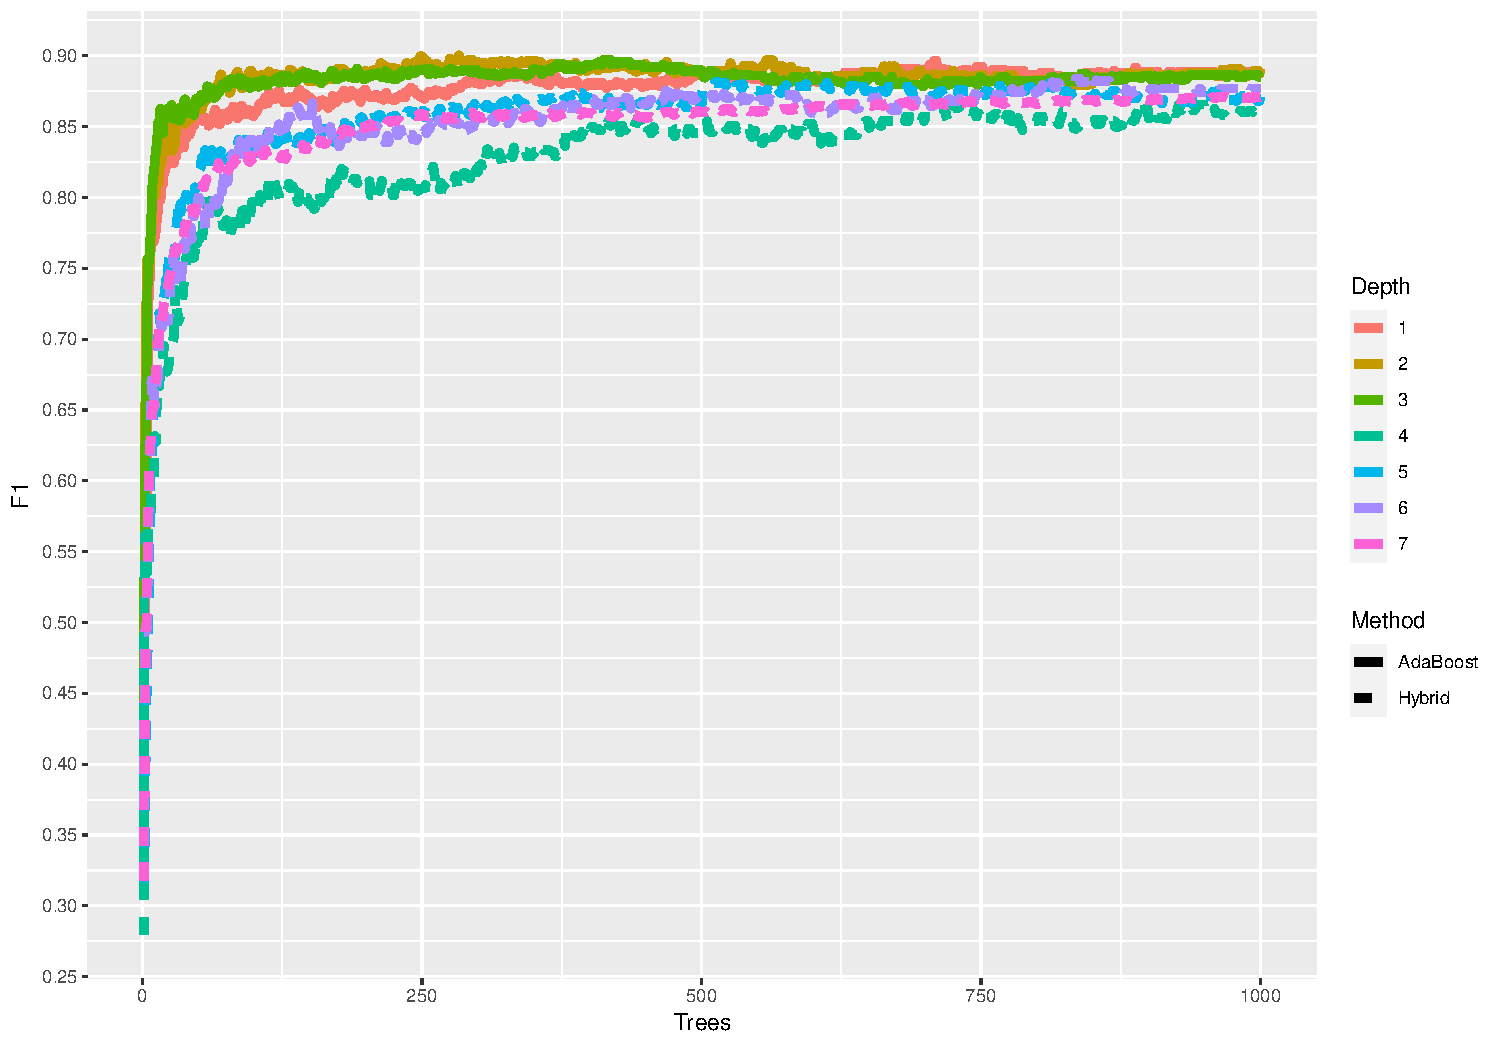
\includegraphics[width=0.8\textwidth]{media/depth.pdf}}
    \caption{
        \raggedright
        A comparison of F1 scores across different max tree depths, methods and forest size.\label{depth_cmp}
    }
\end{figure}
\section{The impact of feature sources\label{feature-results}}
\chapter{Conclusion}

\bibliographystyle{apacite}
\linespread{1}
\raggedright
\bibliography{references.bib}

\end{document}

\documentclass[12pt]{article}
\usepackage{hyperref} % For links
\usepackage{tikz} % For drawing stuff.
\usepackage{qtree} % For drawing trees (needs tikz).
\usepackage{setspace} % For going between double lines and single.
\usepackage[a4paper, total={5.7in, 8in}]{geometry} % Setting margin.
\usepackage{subfiles} % Splitting work across files.
\usepackage{apacite} % Referencing, duh.

\newcommand{\nr}{{\tt newsreduce.org}}
\newcommand{\pr}{PR}

\newcounter{nodeCdepth}%
\newenvironment{nodeC}%
  {\ifnum\value{nodeCdepth}=0%
     \gdef\listfordirtree{}%
     \let\item\nodeCitem%
    \fi%
    \stepcounter{nodeCdepth}}%
  {\addtocounter{nodeCdepth}{-1}%
   \ifnum\value{nodeCdepth}=0%
     \expandafter\dirtree\expandafter{\listfordirtree}%
   \fi}%
\newcommand{\nodeCitem}[1]{%
  \xdef\listfordirtree{%
    \unexpanded\expandafter{\listfordirtree}%
    .\thenodeCdepth\space\unexpanded{#1}. }%
}%

\algnewcommand\algorithmicforeach{\textbf{for each}}
\algdef{S}[FOR]{ForEach}[1]{\algorithmicforeach\ #1\ \algorithmicdo}

\doublespacing

\title{\nr{}
\\
A personalised and privacy-respecting newsreader}
\author{Seán Healy }
\date{August 2020}

\begin{document}

\maketitle
\begin{abstract}
\noindent A web-based newsreader is designed and implemented using a cocktail
of software engineering, natural language processing and machine
learning techniques.  The newsreader aims to tackle some issues
in the current newsreader space: user privacy concerns, information
overload, advertising influence and low coverage.
\end{abstract}
\section*{Acknowledgements}
I must thank Dr. Kevin Koidl for his valuable advice and
help throughout my dissertation.  I must also thank Visma (my
employer) for granting me three months leave in order to complete
this large project and dissertation.
\tableofcontents

\documentclass[12pt]{article}
\usepackage{hyperref} % For links
\usepackage{tikz} % For drawing stuff.
\usepackage{qtree} % For drawing trees (needs tikz).
\usepackage{setspace} % For going between double lines and single.
\usepackage[a4paper, total={5.7in, 8in}]{geometry} % Setting margin.
\usepackage{subfiles} % Splitting work across files.
\usepackage{apacite} % Referencing, duh.

\include{shortcuts}

\doublespacing

\title{\nr{}
\\
A personalised and privacy-respecting newsreader}
\author{Seán Healy }
\date{August 2020}

\begin{document}

\maketitle
\include{abstract}
\include{acknowledge}
\tableofcontents

\include{1-intro/main}
\include{2-background/main}
\include{3-method/main}
\include{4-results}
\include{5-conclusion}

\bibliographystyle{apacite}
\linespread{1}
\raggedright
\bibliography{references.bib}

\end{document}

\documentclass[12pt]{article}
\usepackage{hyperref} % For links
\usepackage{tikz} % For drawing stuff.
\usepackage{qtree} % For drawing trees (needs tikz).
\usepackage{setspace} % For going between double lines and single.
\usepackage[a4paper, total={5.7in, 8in}]{geometry} % Setting margin.
\usepackage{subfiles} % Splitting work across files.
\usepackage{apacite} % Referencing, duh.

\include{shortcuts}

\doublespacing

\title{\nr{}
\\
A personalised and privacy-respecting newsreader}
\author{Seán Healy }
\date{August 2020}

\begin{document}

\maketitle
\include{abstract}
\include{acknowledge}
\tableofcontents

\include{1-intro/main}
\include{2-background/main}
\include{3-method/main}
\include{4-results}
\include{5-conclusion}

\bibliographystyle{apacite}
\linespread{1}
\raggedright
\bibliography{references.bib}

\end{document}

\documentclass[12pt]{article}
\usepackage{hyperref} % For links
\usepackage{tikz} % For drawing stuff.
\usepackage{qtree} % For drawing trees (needs tikz).
\usepackage{setspace} % For going between double lines and single.
\usepackage[a4paper, total={5.7in, 8in}]{geometry} % Setting margin.
\usepackage{subfiles} % Splitting work across files.
\usepackage{apacite} % Referencing, duh.

\include{shortcuts}

\doublespacing

\title{\nr{}
\\
A personalised and privacy-respecting newsreader}
\author{Seán Healy }
\date{August 2020}

\begin{document}

\maketitle
\include{abstract}
\include{acknowledge}
\tableofcontents

\include{1-intro/main}
\include{2-background/main}
\include{3-method/main}
\include{4-results}
\include{5-conclusion}

\bibliographystyle{apacite}
\linespread{1}
\raggedright
\bibliography{references.bib}

\end{document}

\chapter{Results and discussion\label{results}}
\section{Comparison of resource models\label{model-results}}
\section{Comparison of classifiers\label{classifier-results}}
\begin{figure}[H]
    \centering
    \fbox{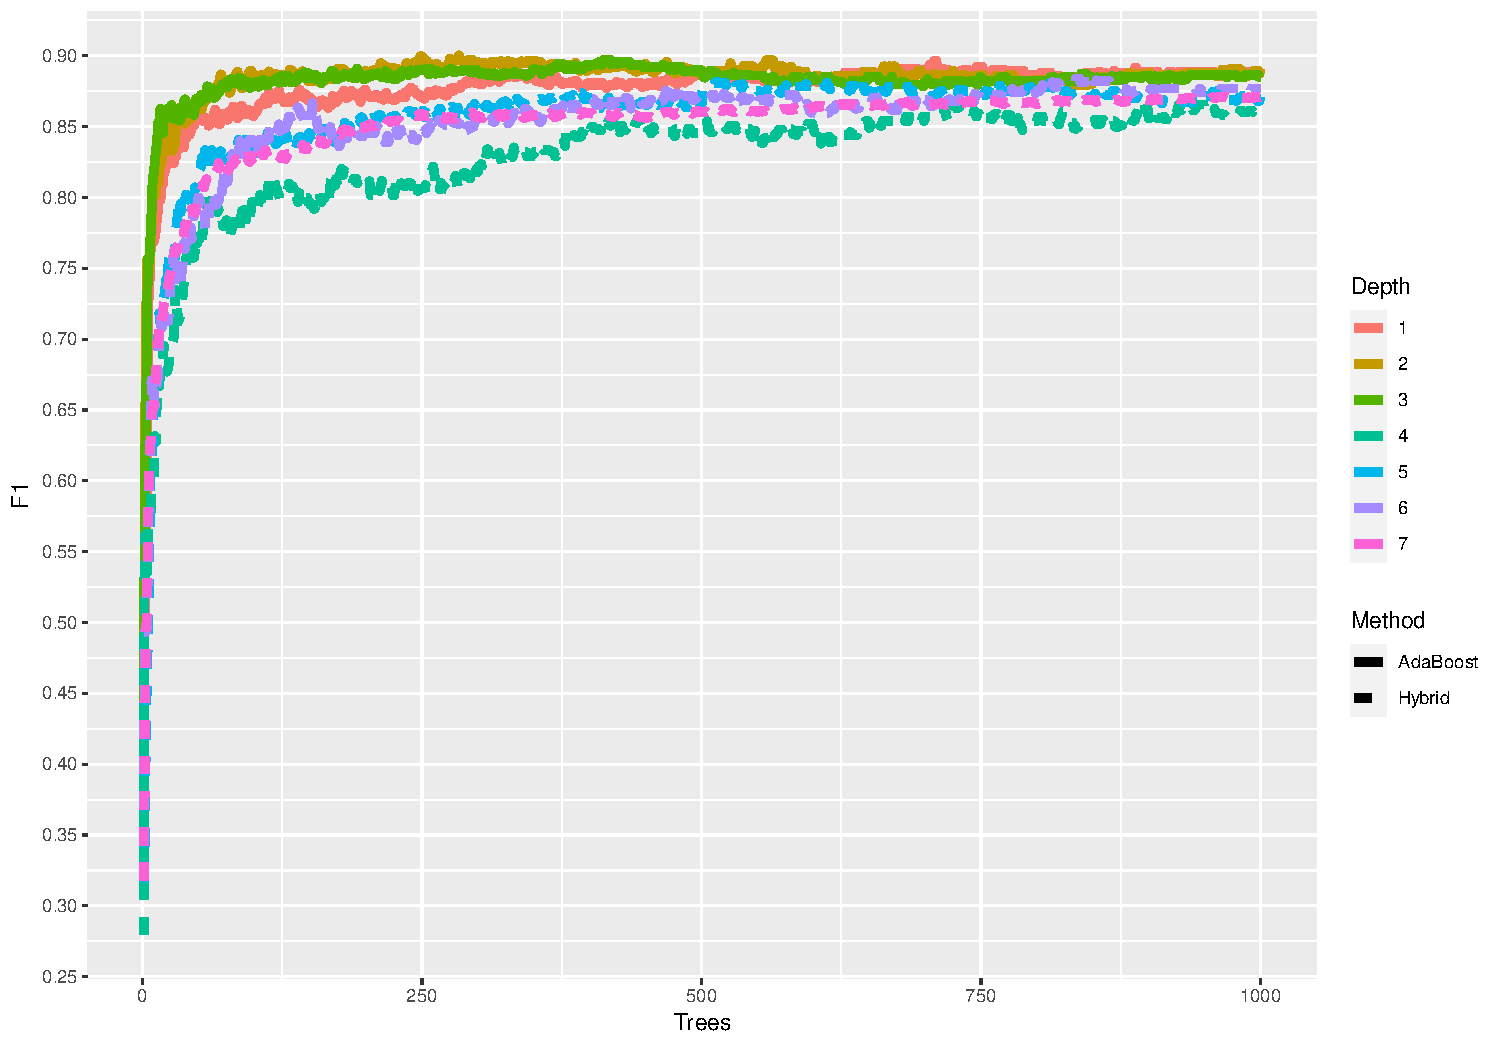
\includegraphics[width=0.8\textwidth]{media/depth.pdf}}
    \caption{
        \raggedright
        A comparison of F1 scores across different max tree depths, methods and forest size.\label{depth_cmp}
    }
\end{figure}
\section{The impact of feature sources\label{feature-results}}
\chapter{Conclusion}

\bibliographystyle{apacite}
\linespread{1}
\raggedright
\bibliography{references.bib}

\end{document}

\documentclass[12pt]{article}
\usepackage{hyperref} % For links
\usepackage{tikz} % For drawing stuff.
\usepackage{qtree} % For drawing trees (needs tikz).
\usepackage{setspace} % For going between double lines and single.
\usepackage[a4paper, total={5.7in, 8in}]{geometry} % Setting margin.
\usepackage{subfiles} % Splitting work across files.
\usepackage{apacite} % Referencing, duh.

\newcommand{\nr}{{\tt newsreduce.org}}
\newcommand{\pr}{PR}

\newcounter{nodeCdepth}%
\newenvironment{nodeC}%
  {\ifnum\value{nodeCdepth}=0%
     \gdef\listfordirtree{}%
     \let\item\nodeCitem%
    \fi%
    \stepcounter{nodeCdepth}}%
  {\addtocounter{nodeCdepth}{-1}%
   \ifnum\value{nodeCdepth}=0%
     \expandafter\dirtree\expandafter{\listfordirtree}%
   \fi}%
\newcommand{\nodeCitem}[1]{%
  \xdef\listfordirtree{%
    \unexpanded\expandafter{\listfordirtree}%
    .\thenodeCdepth\space\unexpanded{#1}. }%
}%

\algnewcommand\algorithmicforeach{\textbf{for each}}
\algdef{S}[FOR]{ForEach}[1]{\algorithmicforeach\ #1\ \algorithmicdo}

\doublespacing

\title{\nr{}
\\
A personalised and privacy-respecting newsreader}
\author{Seán Healy }
\date{August 2020}

\begin{document}

\maketitle
\begin{abstract}
\noindent A web-based newsreader is designed and implemented using a cocktail
of software engineering, natural language processing and machine
learning techniques.  The newsreader aims to tackle some issues
in the current newsreader space: user privacy concerns, information
overload, advertising influence and low coverage.
\end{abstract}
\section*{Acknowledgements}
I must thank Dr. Kevin Koidl for his valuable advice and
help throughout my dissertation.  I must also thank Visma (my
employer) for granting me three months leave in order to complete
this large project and dissertation.
\tableofcontents

\documentclass[12pt]{article}
\usepackage{hyperref} % For links
\usepackage{tikz} % For drawing stuff.
\usepackage{qtree} % For drawing trees (needs tikz).
\usepackage{setspace} % For going between double lines and single.
\usepackage[a4paper, total={5.7in, 8in}]{geometry} % Setting margin.
\usepackage{subfiles} % Splitting work across files.
\usepackage{apacite} % Referencing, duh.

\include{shortcuts}

\doublespacing

\title{\nr{}
\\
A personalised and privacy-respecting newsreader}
\author{Seán Healy }
\date{August 2020}

\begin{document}

\maketitle
\include{abstract}
\include{acknowledge}
\tableofcontents

\include{1-intro/main}
\include{2-background/main}
\include{3-method/main}
\include{4-results}
\include{5-conclusion}

\bibliographystyle{apacite}
\linespread{1}
\raggedright
\bibliography{references.bib}

\end{document}

\documentclass[12pt]{article}
\usepackage{hyperref} % For links
\usepackage{tikz} % For drawing stuff.
\usepackage{qtree} % For drawing trees (needs tikz).
\usepackage{setspace} % For going between double lines and single.
\usepackage[a4paper, total={5.7in, 8in}]{geometry} % Setting margin.
\usepackage{subfiles} % Splitting work across files.
\usepackage{apacite} % Referencing, duh.

\include{shortcuts}

\doublespacing

\title{\nr{}
\\
A personalised and privacy-respecting newsreader}
\author{Seán Healy }
\date{August 2020}

\begin{document}

\maketitle
\include{abstract}
\include{acknowledge}
\tableofcontents

\include{1-intro/main}
\include{2-background/main}
\include{3-method/main}
\include{4-results}
\include{5-conclusion}

\bibliographystyle{apacite}
\linespread{1}
\raggedright
\bibliography{references.bib}

\end{document}

\documentclass[12pt]{article}
\usepackage{hyperref} % For links
\usepackage{tikz} % For drawing stuff.
\usepackage{qtree} % For drawing trees (needs tikz).
\usepackage{setspace} % For going between double lines and single.
\usepackage[a4paper, total={5.7in, 8in}]{geometry} % Setting margin.
\usepackage{subfiles} % Splitting work across files.
\usepackage{apacite} % Referencing, duh.

\include{shortcuts}

\doublespacing

\title{\nr{}
\\
A personalised and privacy-respecting newsreader}
\author{Seán Healy }
\date{August 2020}

\begin{document}

\maketitle
\include{abstract}
\include{acknowledge}
\tableofcontents

\include{1-intro/main}
\include{2-background/main}
\include{3-method/main}
\include{4-results}
\include{5-conclusion}

\bibliographystyle{apacite}
\linespread{1}
\raggedright
\bibliography{references.bib}

\end{document}

\chapter{Results and discussion\label{results}}
\section{Comparison of resource models\label{model-results}}
\section{Comparison of classifiers\label{classifier-results}}
\begin{figure}[H]
    \centering
    \fbox{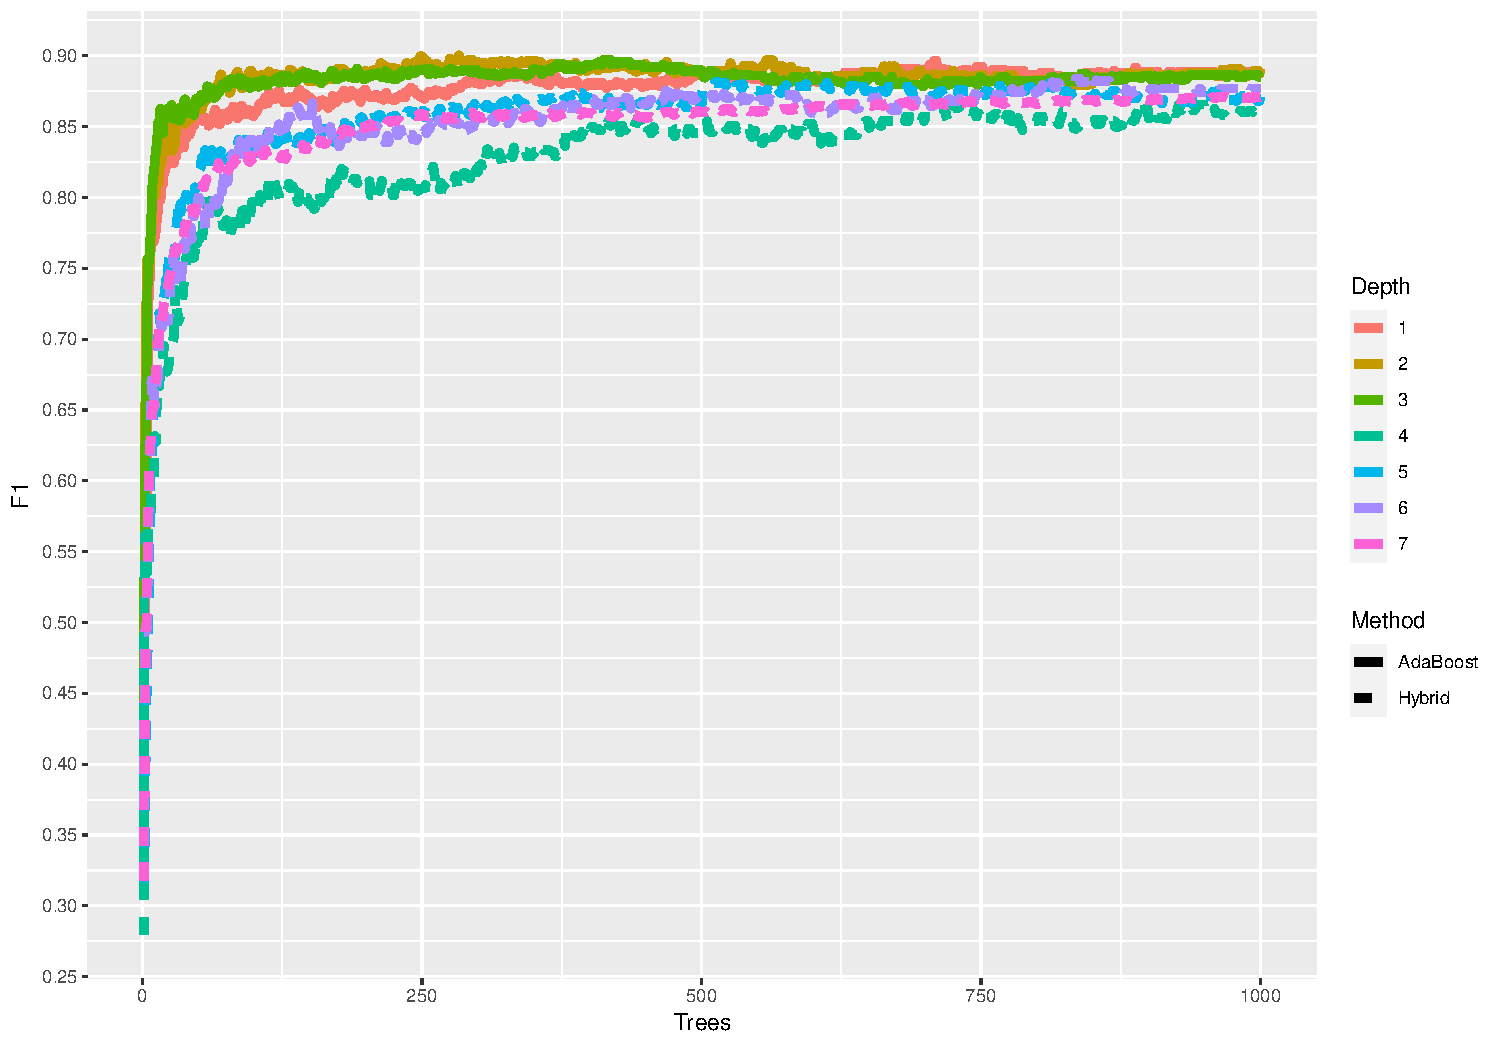
\includegraphics[width=0.8\textwidth]{media/depth.pdf}}
    \caption{
        \raggedright
        A comparison of F1 scores across different max tree depths, methods and forest size.\label{depth_cmp}
    }
\end{figure}
\section{The impact of feature sources\label{feature-results}}
\chapter{Conclusion}

\bibliographystyle{apacite}
\linespread{1}
\raggedright
\bibliography{references.bib}

\end{document}

\chapter{Results and discussion\label{results}}
\section{Comparison of resource models\label{model-results}}
\section{Comparison of classifiers\label{classifier-results}}
\begin{figure}[H]
    \centering
    \fbox{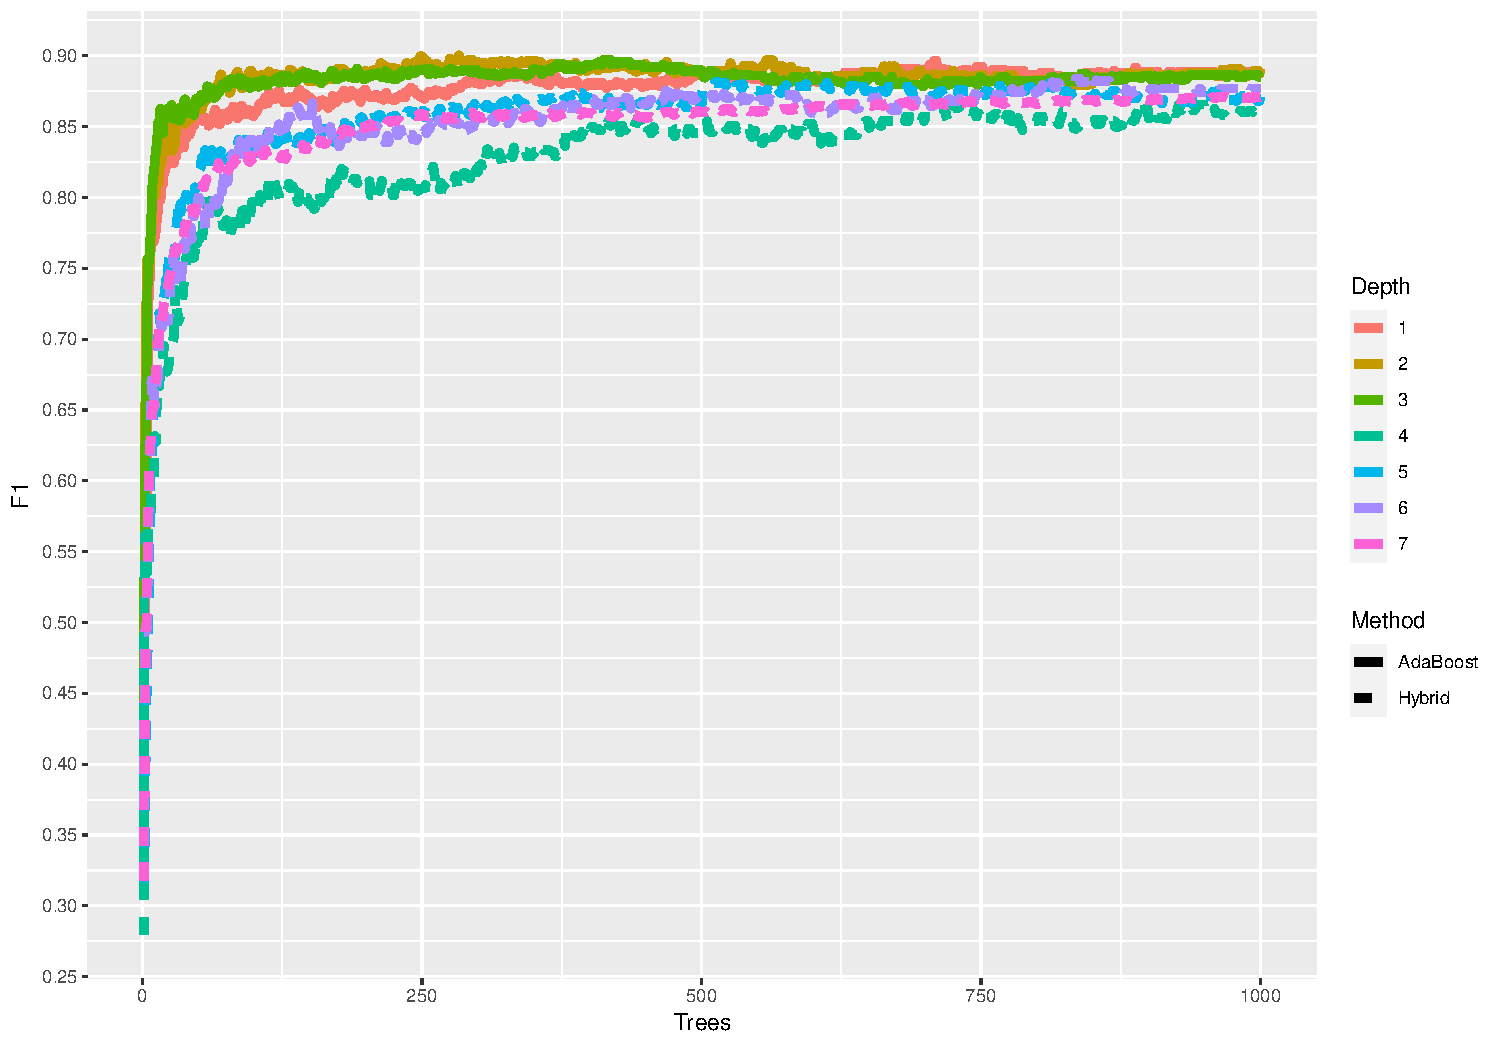
\includegraphics[width=0.8\textwidth]{media/depth.pdf}}
    \caption{
        \raggedright
        A comparison of F1 scores across different max tree depths, methods and forest size.\label{depth_cmp}
    }
\end{figure}
\section{The impact of feature sources\label{feature-results}}
\chapter{Conclusion}

\bibliographystyle{apacite}
\linespread{1}
\raggedright
\bibliography{references.bib}

\end{document}

\documentclass[12pt]{article}
\usepackage{hyperref} % For links
\usepackage{tikz} % For drawing stuff.
\usepackage{qtree} % For drawing trees (needs tikz).
\usepackage{setspace} % For going between double lines and single.
\usepackage[a4paper, total={5.7in, 8in}]{geometry} % Setting margin.
\usepackage{subfiles} % Splitting work across files.
\usepackage{apacite} % Referencing, duh.

\newcommand{\nr}{{\tt newsreduce.org}}
\newcommand{\pr}{PR}

\newcounter{nodeCdepth}%
\newenvironment{nodeC}%
  {\ifnum\value{nodeCdepth}=0%
     \gdef\listfordirtree{}%
     \let\item\nodeCitem%
    \fi%
    \stepcounter{nodeCdepth}}%
  {\addtocounter{nodeCdepth}{-1}%
   \ifnum\value{nodeCdepth}=0%
     \expandafter\dirtree\expandafter{\listfordirtree}%
   \fi}%
\newcommand{\nodeCitem}[1]{%
  \xdef\listfordirtree{%
    \unexpanded\expandafter{\listfordirtree}%
    .\thenodeCdepth\space\unexpanded{#1}. }%
}%

\algnewcommand\algorithmicforeach{\textbf{for each}}
\algdef{S}[FOR]{ForEach}[1]{\algorithmicforeach\ #1\ \algorithmicdo}

\doublespacing

\title{\nr{}
\\
A personalised and privacy-respecting newsreader}
\author{Seán Healy }
\date{August 2020}

\begin{document}

\maketitle
\begin{abstract}
\noindent A web-based newsreader is designed and implemented using a cocktail
of software engineering, natural language processing and machine
learning techniques.  The newsreader aims to tackle some issues
in the current newsreader space: user privacy concerns, information
overload, advertising influence and low coverage.
\end{abstract}
\section*{Acknowledgements}
I must thank Dr. Kevin Koidl for his valuable advice and
help throughout my dissertation.  I must also thank Visma (my
employer) for granting me three months leave in order to complete
this large project and dissertation.
\tableofcontents

\documentclass[12pt]{article}
\usepackage{hyperref} % For links
\usepackage{tikz} % For drawing stuff.
\usepackage{qtree} % For drawing trees (needs tikz).
\usepackage{setspace} % For going between double lines and single.
\usepackage[a4paper, total={5.7in, 8in}]{geometry} % Setting margin.
\usepackage{subfiles} % Splitting work across files.
\usepackage{apacite} % Referencing, duh.

\newcommand{\nr}{{\tt newsreduce.org}}
\newcommand{\pr}{PR}

\newcounter{nodeCdepth}%
\newenvironment{nodeC}%
  {\ifnum\value{nodeCdepth}=0%
     \gdef\listfordirtree{}%
     \let\item\nodeCitem%
    \fi%
    \stepcounter{nodeCdepth}}%
  {\addtocounter{nodeCdepth}{-1}%
   \ifnum\value{nodeCdepth}=0%
     \expandafter\dirtree\expandafter{\listfordirtree}%
   \fi}%
\newcommand{\nodeCitem}[1]{%
  \xdef\listfordirtree{%
    \unexpanded\expandafter{\listfordirtree}%
    .\thenodeCdepth\space\unexpanded{#1}. }%
}%

\algnewcommand\algorithmicforeach{\textbf{for each}}
\algdef{S}[FOR]{ForEach}[1]{\algorithmicforeach\ #1\ \algorithmicdo}

\doublespacing

\title{\nr{}
\\
A personalised and privacy-respecting newsreader}
\author{Seán Healy }
\date{August 2020}

\begin{document}

\maketitle
\begin{abstract}
\noindent A web-based newsreader is designed and implemented using a cocktail
of software engineering, natural language processing and machine
learning techniques.  The newsreader aims to tackle some issues
in the current newsreader space: user privacy concerns, information
overload, advertising influence and low coverage.
\end{abstract}
\section*{Acknowledgements}
I must thank Dr. Kevin Koidl for his valuable advice and
help throughout my dissertation.  I must also thank Visma (my
employer) for granting me three months leave in order to complete
this large project and dissertation.
\tableofcontents

\documentclass[12pt]{article}
\usepackage{hyperref} % For links
\usepackage{tikz} % For drawing stuff.
\usepackage{qtree} % For drawing trees (needs tikz).
\usepackage{setspace} % For going between double lines and single.
\usepackage[a4paper, total={5.7in, 8in}]{geometry} % Setting margin.
\usepackage{subfiles} % Splitting work across files.
\usepackage{apacite} % Referencing, duh.

\include{shortcuts}

\doublespacing

\title{\nr{}
\\
A personalised and privacy-respecting newsreader}
\author{Seán Healy }
\date{August 2020}

\begin{document}

\maketitle
\include{abstract}
\include{acknowledge}
\tableofcontents

\include{1-intro/main}
\include{2-background/main}
\include{3-method/main}
\include{4-results}
\include{5-conclusion}

\bibliographystyle{apacite}
\linespread{1}
\raggedright
\bibliography{references.bib}

\end{document}

\documentclass[12pt]{article}
\usepackage{hyperref} % For links
\usepackage{tikz} % For drawing stuff.
\usepackage{qtree} % For drawing trees (needs tikz).
\usepackage{setspace} % For going between double lines and single.
\usepackage[a4paper, total={5.7in, 8in}]{geometry} % Setting margin.
\usepackage{subfiles} % Splitting work across files.
\usepackage{apacite} % Referencing, duh.

\include{shortcuts}

\doublespacing

\title{\nr{}
\\
A personalised and privacy-respecting newsreader}
\author{Seán Healy }
\date{August 2020}

\begin{document}

\maketitle
\include{abstract}
\include{acknowledge}
\tableofcontents

\include{1-intro/main}
\include{2-background/main}
\include{3-method/main}
\include{4-results}
\include{5-conclusion}

\bibliographystyle{apacite}
\linespread{1}
\raggedright
\bibliography{references.bib}

\end{document}

\documentclass[12pt]{article}
\usepackage{hyperref} % For links
\usepackage{tikz} % For drawing stuff.
\usepackage{qtree} % For drawing trees (needs tikz).
\usepackage{setspace} % For going between double lines and single.
\usepackage[a4paper, total={5.7in, 8in}]{geometry} % Setting margin.
\usepackage{subfiles} % Splitting work across files.
\usepackage{apacite} % Referencing, duh.

\include{shortcuts}

\doublespacing

\title{\nr{}
\\
A personalised and privacy-respecting newsreader}
\author{Seán Healy }
\date{August 2020}

\begin{document}

\maketitle
\include{abstract}
\include{acknowledge}
\tableofcontents

\include{1-intro/main}
\include{2-background/main}
\include{3-method/main}
\include{4-results}
\include{5-conclusion}

\bibliographystyle{apacite}
\linespread{1}
\raggedright
\bibliography{references.bib}

\end{document}

\chapter{Results and discussion\label{results}}
\section{Comparison of resource models\label{model-results}}
\section{Comparison of classifiers\label{classifier-results}}
\begin{figure}[H]
    \centering
    \fbox{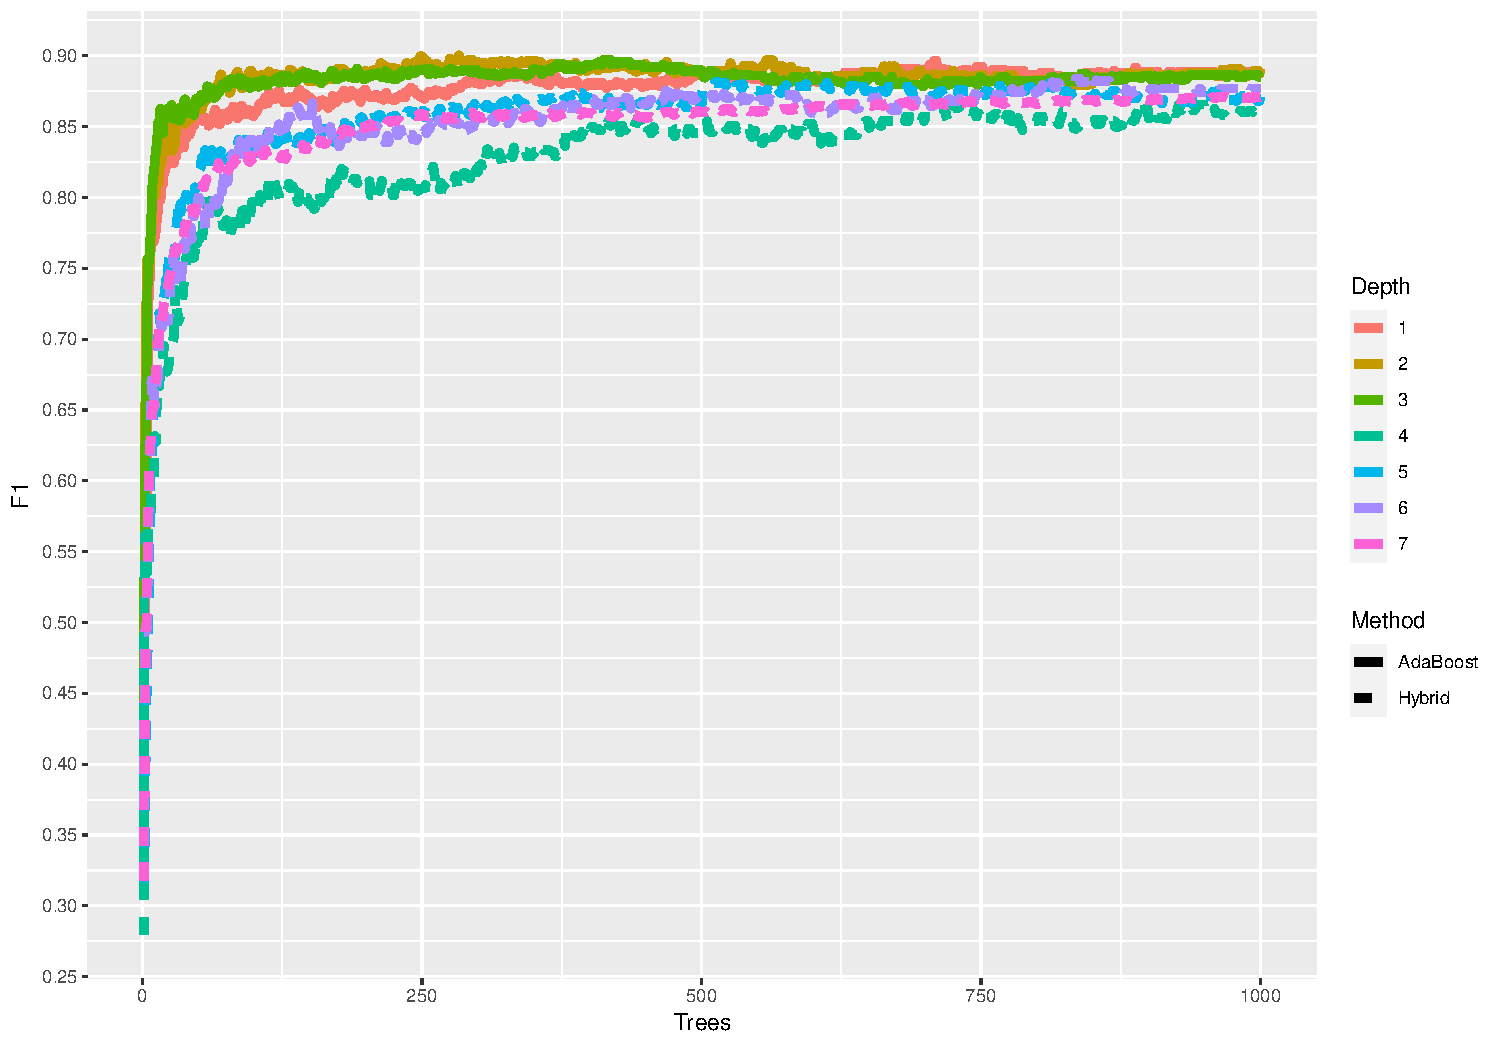
\includegraphics[width=0.8\textwidth]{media/depth.pdf}}
    \caption{
        \raggedright
        A comparison of F1 scores across different max tree depths, methods and forest size.\label{depth_cmp}
    }
\end{figure}
\section{The impact of feature sources\label{feature-results}}
\chapter{Conclusion}

\bibliographystyle{apacite}
\linespread{1}
\raggedright
\bibliography{references.bib}

\end{document}

\documentclass[12pt]{article}
\usepackage{hyperref} % For links
\usepackage{tikz} % For drawing stuff.
\usepackage{qtree} % For drawing trees (needs tikz).
\usepackage{setspace} % For going between double lines and single.
\usepackage[a4paper, total={5.7in, 8in}]{geometry} % Setting margin.
\usepackage{subfiles} % Splitting work across files.
\usepackage{apacite} % Referencing, duh.

\newcommand{\nr}{{\tt newsreduce.org}}
\newcommand{\pr}{PR}

\newcounter{nodeCdepth}%
\newenvironment{nodeC}%
  {\ifnum\value{nodeCdepth}=0%
     \gdef\listfordirtree{}%
     \let\item\nodeCitem%
    \fi%
    \stepcounter{nodeCdepth}}%
  {\addtocounter{nodeCdepth}{-1}%
   \ifnum\value{nodeCdepth}=0%
     \expandafter\dirtree\expandafter{\listfordirtree}%
   \fi}%
\newcommand{\nodeCitem}[1]{%
  \xdef\listfordirtree{%
    \unexpanded\expandafter{\listfordirtree}%
    .\thenodeCdepth\space\unexpanded{#1}. }%
}%

\algnewcommand\algorithmicforeach{\textbf{for each}}
\algdef{S}[FOR]{ForEach}[1]{\algorithmicforeach\ #1\ \algorithmicdo}

\doublespacing

\title{\nr{}
\\
A personalised and privacy-respecting newsreader}
\author{Seán Healy }
\date{August 2020}

\begin{document}

\maketitle
\begin{abstract}
\noindent A web-based newsreader is designed and implemented using a cocktail
of software engineering, natural language processing and machine
learning techniques.  The newsreader aims to tackle some issues
in the current newsreader space: user privacy concerns, information
overload, advertising influence and low coverage.
\end{abstract}
\section*{Acknowledgements}
I must thank Dr. Kevin Koidl for his valuable advice and
help throughout my dissertation.  I must also thank Visma (my
employer) for granting me three months leave in order to complete
this large project and dissertation.
\tableofcontents

\documentclass[12pt]{article}
\usepackage{hyperref} % For links
\usepackage{tikz} % For drawing stuff.
\usepackage{qtree} % For drawing trees (needs tikz).
\usepackage{setspace} % For going between double lines and single.
\usepackage[a4paper, total={5.7in, 8in}]{geometry} % Setting margin.
\usepackage{subfiles} % Splitting work across files.
\usepackage{apacite} % Referencing, duh.

\include{shortcuts}

\doublespacing

\title{\nr{}
\\
A personalised and privacy-respecting newsreader}
\author{Seán Healy }
\date{August 2020}

\begin{document}

\maketitle
\include{abstract}
\include{acknowledge}
\tableofcontents

\include{1-intro/main}
\include{2-background/main}
\include{3-method/main}
\include{4-results}
\include{5-conclusion}

\bibliographystyle{apacite}
\linespread{1}
\raggedright
\bibliography{references.bib}

\end{document}

\documentclass[12pt]{article}
\usepackage{hyperref} % For links
\usepackage{tikz} % For drawing stuff.
\usepackage{qtree} % For drawing trees (needs tikz).
\usepackage{setspace} % For going between double lines and single.
\usepackage[a4paper, total={5.7in, 8in}]{geometry} % Setting margin.
\usepackage{subfiles} % Splitting work across files.
\usepackage{apacite} % Referencing, duh.

\include{shortcuts}

\doublespacing

\title{\nr{}
\\
A personalised and privacy-respecting newsreader}
\author{Seán Healy }
\date{August 2020}

\begin{document}

\maketitle
\include{abstract}
\include{acknowledge}
\tableofcontents

\include{1-intro/main}
\include{2-background/main}
\include{3-method/main}
\include{4-results}
\include{5-conclusion}

\bibliographystyle{apacite}
\linespread{1}
\raggedright
\bibliography{references.bib}

\end{document}

\documentclass[12pt]{article}
\usepackage{hyperref} % For links
\usepackage{tikz} % For drawing stuff.
\usepackage{qtree} % For drawing trees (needs tikz).
\usepackage{setspace} % For going between double lines and single.
\usepackage[a4paper, total={5.7in, 8in}]{geometry} % Setting margin.
\usepackage{subfiles} % Splitting work across files.
\usepackage{apacite} % Referencing, duh.

\include{shortcuts}

\doublespacing

\title{\nr{}
\\
A personalised and privacy-respecting newsreader}
\author{Seán Healy }
\date{August 2020}

\begin{document}

\maketitle
\include{abstract}
\include{acknowledge}
\tableofcontents

\include{1-intro/main}
\include{2-background/main}
\include{3-method/main}
\include{4-results}
\include{5-conclusion}

\bibliographystyle{apacite}
\linespread{1}
\raggedright
\bibliography{references.bib}

\end{document}

\chapter{Results and discussion\label{results}}
\section{Comparison of resource models\label{model-results}}
\section{Comparison of classifiers\label{classifier-results}}
\begin{figure}[H]
    \centering
    \fbox{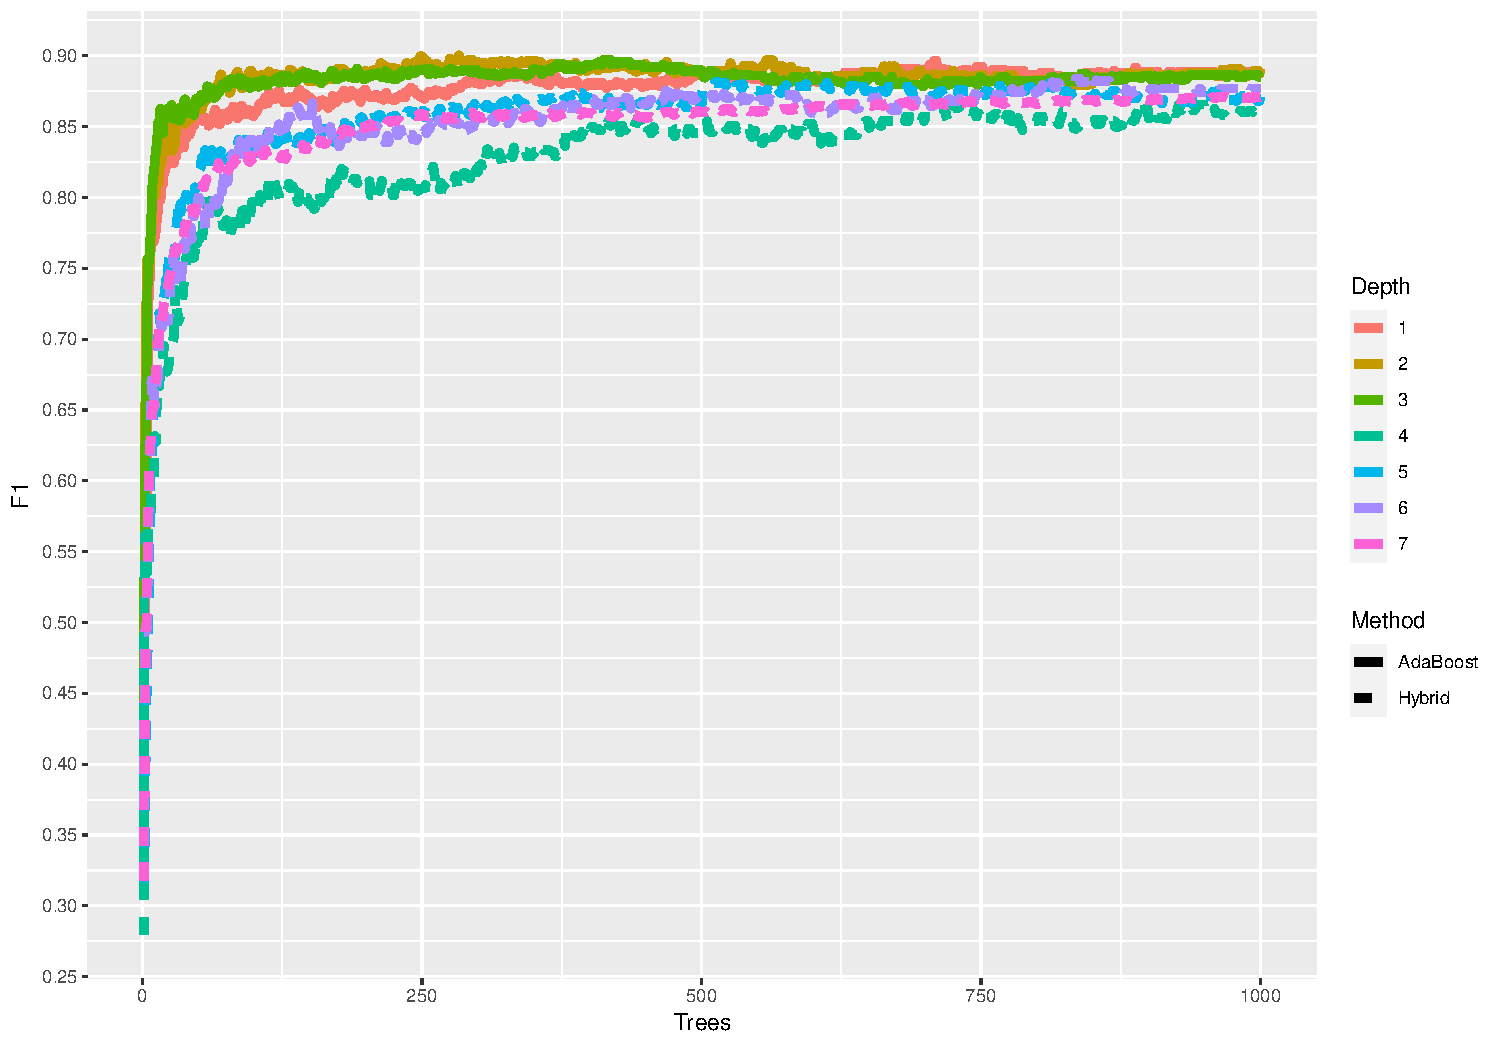
\includegraphics[width=0.8\textwidth]{media/depth.pdf}}
    \caption{
        \raggedright
        A comparison of F1 scores across different max tree depths, methods and forest size.\label{depth_cmp}
    }
\end{figure}
\section{The impact of feature sources\label{feature-results}}
\chapter{Conclusion}

\bibliographystyle{apacite}
\linespread{1}
\raggedright
\bibliography{references.bib}

\end{document}

\documentclass[12pt]{article}
\usepackage{hyperref} % For links
\usepackage{tikz} % For drawing stuff.
\usepackage{qtree} % For drawing trees (needs tikz).
\usepackage{setspace} % For going between double lines and single.
\usepackage[a4paper, total={5.7in, 8in}]{geometry} % Setting margin.
\usepackage{subfiles} % Splitting work across files.
\usepackage{apacite} % Referencing, duh.

\newcommand{\nr}{{\tt newsreduce.org}}
\newcommand{\pr}{PR}

\newcounter{nodeCdepth}%
\newenvironment{nodeC}%
  {\ifnum\value{nodeCdepth}=0%
     \gdef\listfordirtree{}%
     \let\item\nodeCitem%
    \fi%
    \stepcounter{nodeCdepth}}%
  {\addtocounter{nodeCdepth}{-1}%
   \ifnum\value{nodeCdepth}=0%
     \expandafter\dirtree\expandafter{\listfordirtree}%
   \fi}%
\newcommand{\nodeCitem}[1]{%
  \xdef\listfordirtree{%
    \unexpanded\expandafter{\listfordirtree}%
    .\thenodeCdepth\space\unexpanded{#1}. }%
}%

\algnewcommand\algorithmicforeach{\textbf{for each}}
\algdef{S}[FOR]{ForEach}[1]{\algorithmicforeach\ #1\ \algorithmicdo}

\doublespacing

\title{\nr{}
\\
A personalised and privacy-respecting newsreader}
\author{Seán Healy }
\date{August 2020}

\begin{document}

\maketitle
\begin{abstract}
\noindent A web-based newsreader is designed and implemented using a cocktail
of software engineering, natural language processing and machine
learning techniques.  The newsreader aims to tackle some issues
in the current newsreader space: user privacy concerns, information
overload, advertising influence and low coverage.
\end{abstract}
\section*{Acknowledgements}
I must thank Dr. Kevin Koidl for his valuable advice and
help throughout my dissertation.  I must also thank Visma (my
employer) for granting me three months leave in order to complete
this large project and dissertation.
\tableofcontents

\documentclass[12pt]{article}
\usepackage{hyperref} % For links
\usepackage{tikz} % For drawing stuff.
\usepackage{qtree} % For drawing trees (needs tikz).
\usepackage{setspace} % For going between double lines and single.
\usepackage[a4paper, total={5.7in, 8in}]{geometry} % Setting margin.
\usepackage{subfiles} % Splitting work across files.
\usepackage{apacite} % Referencing, duh.

\include{shortcuts}

\doublespacing

\title{\nr{}
\\
A personalised and privacy-respecting newsreader}
\author{Seán Healy }
\date{August 2020}

\begin{document}

\maketitle
\include{abstract}
\include{acknowledge}
\tableofcontents

\include{1-intro/main}
\include{2-background/main}
\include{3-method/main}
\include{4-results}
\include{5-conclusion}

\bibliographystyle{apacite}
\linespread{1}
\raggedright
\bibliography{references.bib}

\end{document}

\documentclass[12pt]{article}
\usepackage{hyperref} % For links
\usepackage{tikz} % For drawing stuff.
\usepackage{qtree} % For drawing trees (needs tikz).
\usepackage{setspace} % For going between double lines and single.
\usepackage[a4paper, total={5.7in, 8in}]{geometry} % Setting margin.
\usepackage{subfiles} % Splitting work across files.
\usepackage{apacite} % Referencing, duh.

\include{shortcuts}

\doublespacing

\title{\nr{}
\\
A personalised and privacy-respecting newsreader}
\author{Seán Healy }
\date{August 2020}

\begin{document}

\maketitle
\include{abstract}
\include{acknowledge}
\tableofcontents

\include{1-intro/main}
\include{2-background/main}
\include{3-method/main}
\include{4-results}
\include{5-conclusion}

\bibliographystyle{apacite}
\linespread{1}
\raggedright
\bibliography{references.bib}

\end{document}

\documentclass[12pt]{article}
\usepackage{hyperref} % For links
\usepackage{tikz} % For drawing stuff.
\usepackage{qtree} % For drawing trees (needs tikz).
\usepackage{setspace} % For going between double lines and single.
\usepackage[a4paper, total={5.7in, 8in}]{geometry} % Setting margin.
\usepackage{subfiles} % Splitting work across files.
\usepackage{apacite} % Referencing, duh.

\include{shortcuts}

\doublespacing

\title{\nr{}
\\
A personalised and privacy-respecting newsreader}
\author{Seán Healy }
\date{August 2020}

\begin{document}

\maketitle
\include{abstract}
\include{acknowledge}
\tableofcontents

\include{1-intro/main}
\include{2-background/main}
\include{3-method/main}
\include{4-results}
\include{5-conclusion}

\bibliographystyle{apacite}
\linespread{1}
\raggedright
\bibliography{references.bib}

\end{document}

\chapter{Results and discussion\label{results}}
\section{Comparison of resource models\label{model-results}}
\section{Comparison of classifiers\label{classifier-results}}
\begin{figure}[H]
    \centering
    \fbox{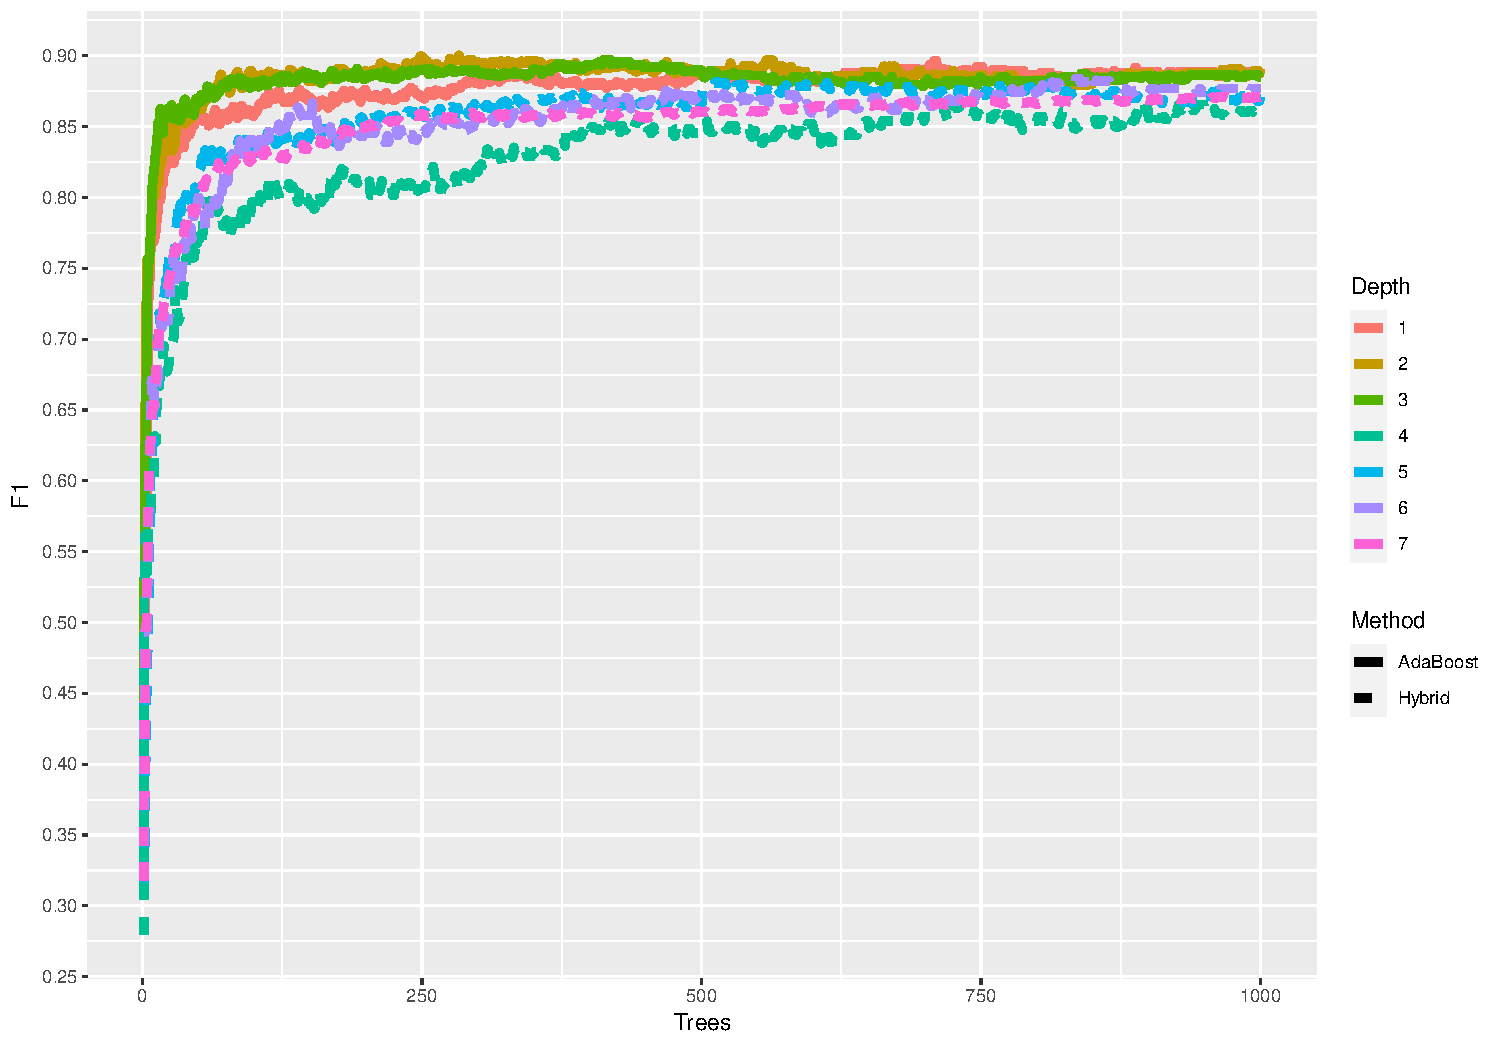
\includegraphics[width=0.8\textwidth]{media/depth.pdf}}
    \caption{
        \raggedright
        A comparison of F1 scores across different max tree depths, methods and forest size.\label{depth_cmp}
    }
\end{figure}
\section{The impact of feature sources\label{feature-results}}
\chapter{Conclusion}

\bibliographystyle{apacite}
\linespread{1}
\raggedright
\bibliography{references.bib}

\end{document}

\chapter{Results and discussion\label{results}}
\section{Comparison of resource models\label{model-results}}
\section{Comparison of classifiers\label{classifier-results}}
\begin{figure}[H]
    \centering
    \fbox{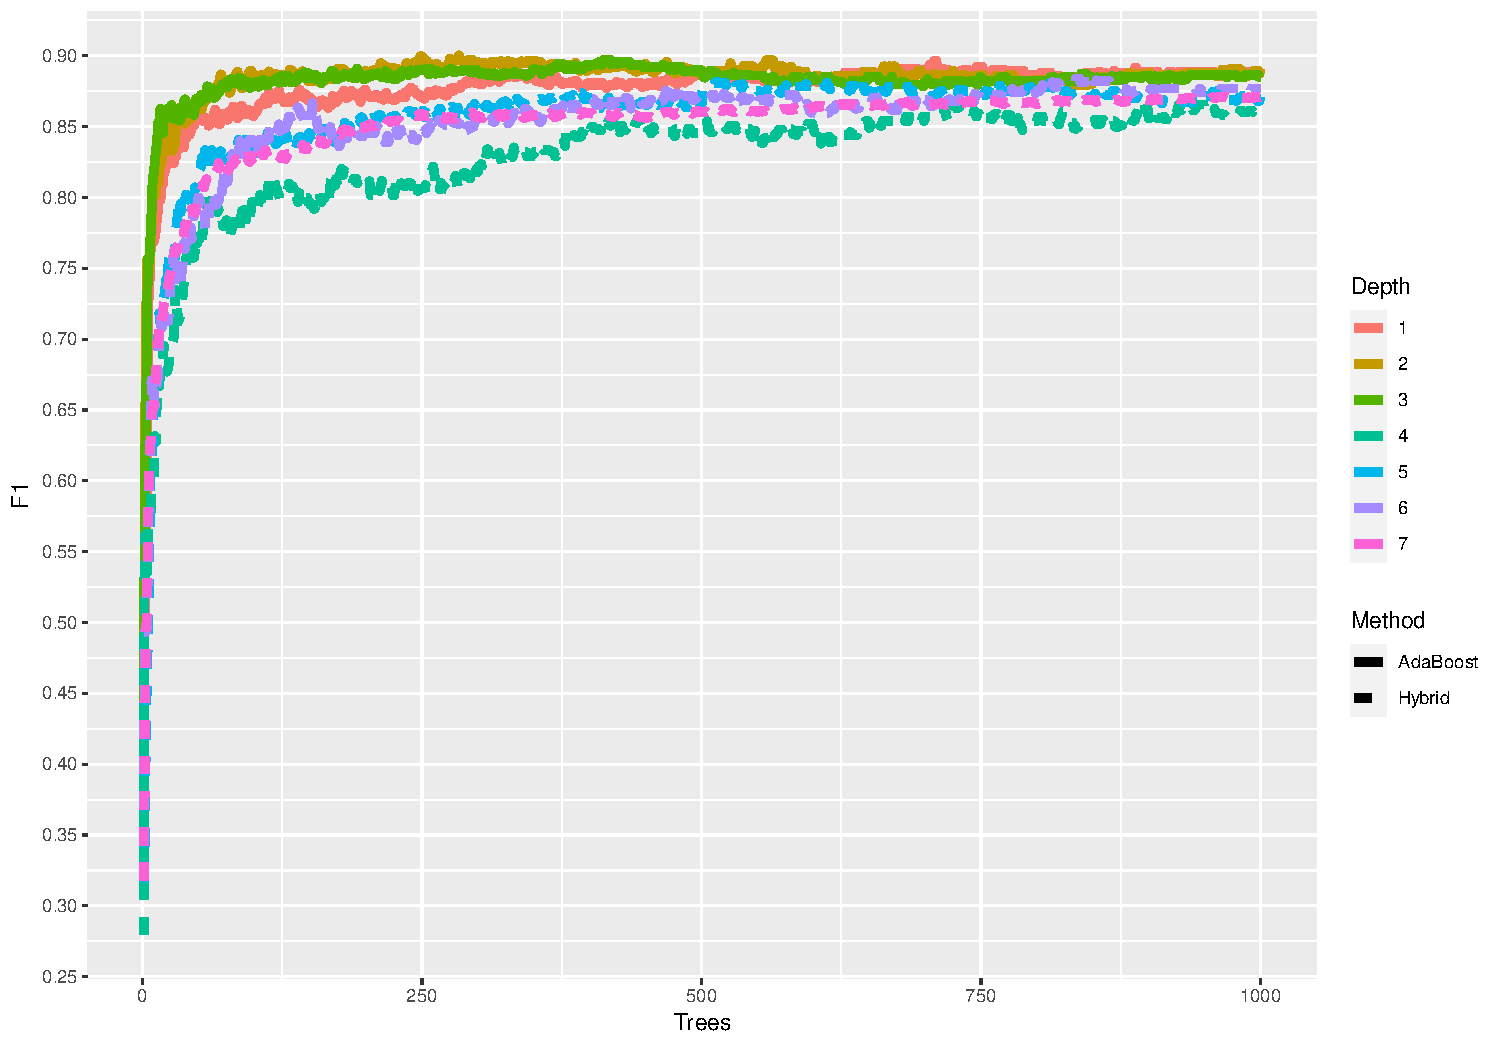
\includegraphics[width=0.8\textwidth]{media/depth.pdf}}
    \caption{
        \raggedright
        A comparison of F1 scores across different max tree depths, methods and forest size.\label{depth_cmp}
    }
\end{figure}
\section{The impact of feature sources\label{feature-results}}
\chapter{Conclusion}

\bibliographystyle{apacite}
\linespread{1}
\raggedright
\bibliography{references.bib}

\end{document}

\documentclass[12pt]{article}
\usepackage{hyperref} % For links
\usepackage{tikz} % For drawing stuff.
\usepackage{qtree} % For drawing trees (needs tikz).
\usepackage{setspace} % For going between double lines and single.
\usepackage[a4paper, total={5.7in, 8in}]{geometry} % Setting margin.
\usepackage{subfiles} % Splitting work across files.
\usepackage{apacite} % Referencing, duh.

\newcommand{\nr}{{\tt newsreduce.org}}
\newcommand{\pr}{PR}

\newcounter{nodeCdepth}%
\newenvironment{nodeC}%
  {\ifnum\value{nodeCdepth}=0%
     \gdef\listfordirtree{}%
     \let\item\nodeCitem%
    \fi%
    \stepcounter{nodeCdepth}}%
  {\addtocounter{nodeCdepth}{-1}%
   \ifnum\value{nodeCdepth}=0%
     \expandafter\dirtree\expandafter{\listfordirtree}%
   \fi}%
\newcommand{\nodeCitem}[1]{%
  \xdef\listfordirtree{%
    \unexpanded\expandafter{\listfordirtree}%
    .\thenodeCdepth\space\unexpanded{#1}. }%
}%

\algnewcommand\algorithmicforeach{\textbf{for each}}
\algdef{S}[FOR]{ForEach}[1]{\algorithmicforeach\ #1\ \algorithmicdo}

\doublespacing

\title{\nr{}
\\
A personalised and privacy-respecting newsreader}
\author{Seán Healy }
\date{August 2020}

\begin{document}

\maketitle
\begin{abstract}
\noindent A web-based newsreader is designed and implemented using a cocktail
of software engineering, natural language processing and machine
learning techniques.  The newsreader aims to tackle some issues
in the current newsreader space: user privacy concerns, information
overload, advertising influence and low coverage.
\end{abstract}
\section*{Acknowledgements}
I must thank Dr. Kevin Koidl for his valuable advice and
help throughout my dissertation.  I must also thank Visma (my
employer) for granting me three months leave in order to complete
this large project and dissertation.
\tableofcontents

\documentclass[12pt]{article}
\usepackage{hyperref} % For links
\usepackage{tikz} % For drawing stuff.
\usepackage{qtree} % For drawing trees (needs tikz).
\usepackage{setspace} % For going between double lines and single.
\usepackage[a4paper, total={5.7in, 8in}]{geometry} % Setting margin.
\usepackage{subfiles} % Splitting work across files.
\usepackage{apacite} % Referencing, duh.

\newcommand{\nr}{{\tt newsreduce.org}}
\newcommand{\pr}{PR}

\newcounter{nodeCdepth}%
\newenvironment{nodeC}%
  {\ifnum\value{nodeCdepth}=0%
     \gdef\listfordirtree{}%
     \let\item\nodeCitem%
    \fi%
    \stepcounter{nodeCdepth}}%
  {\addtocounter{nodeCdepth}{-1}%
   \ifnum\value{nodeCdepth}=0%
     \expandafter\dirtree\expandafter{\listfordirtree}%
   \fi}%
\newcommand{\nodeCitem}[1]{%
  \xdef\listfordirtree{%
    \unexpanded\expandafter{\listfordirtree}%
    .\thenodeCdepth\space\unexpanded{#1}. }%
}%

\algnewcommand\algorithmicforeach{\textbf{for each}}
\algdef{S}[FOR]{ForEach}[1]{\algorithmicforeach\ #1\ \algorithmicdo}

\doublespacing

\title{\nr{}
\\
A personalised and privacy-respecting newsreader}
\author{Seán Healy }
\date{August 2020}

\begin{document}

\maketitle
\begin{abstract}
\noindent A web-based newsreader is designed and implemented using a cocktail
of software engineering, natural language processing and machine
learning techniques.  The newsreader aims to tackle some issues
in the current newsreader space: user privacy concerns, information
overload, advertising influence and low coverage.
\end{abstract}
\section*{Acknowledgements}
I must thank Dr. Kevin Koidl for his valuable advice and
help throughout my dissertation.  I must also thank Visma (my
employer) for granting me three months leave in order to complete
this large project and dissertation.
\tableofcontents

\documentclass[12pt]{article}
\usepackage{hyperref} % For links
\usepackage{tikz} % For drawing stuff.
\usepackage{qtree} % For drawing trees (needs tikz).
\usepackage{setspace} % For going between double lines and single.
\usepackage[a4paper, total={5.7in, 8in}]{geometry} % Setting margin.
\usepackage{subfiles} % Splitting work across files.
\usepackage{apacite} % Referencing, duh.

\include{shortcuts}

\doublespacing

\title{\nr{}
\\
A personalised and privacy-respecting newsreader}
\author{Seán Healy }
\date{August 2020}

\begin{document}

\maketitle
\include{abstract}
\include{acknowledge}
\tableofcontents

\include{1-intro/main}
\include{2-background/main}
\include{3-method/main}
\include{4-results}
\include{5-conclusion}

\bibliographystyle{apacite}
\linespread{1}
\raggedright
\bibliography{references.bib}

\end{document}

\documentclass[12pt]{article}
\usepackage{hyperref} % For links
\usepackage{tikz} % For drawing stuff.
\usepackage{qtree} % For drawing trees (needs tikz).
\usepackage{setspace} % For going between double lines and single.
\usepackage[a4paper, total={5.7in, 8in}]{geometry} % Setting margin.
\usepackage{subfiles} % Splitting work across files.
\usepackage{apacite} % Referencing, duh.

\include{shortcuts}

\doublespacing

\title{\nr{}
\\
A personalised and privacy-respecting newsreader}
\author{Seán Healy }
\date{August 2020}

\begin{document}

\maketitle
\include{abstract}
\include{acknowledge}
\tableofcontents

\include{1-intro/main}
\include{2-background/main}
\include{3-method/main}
\include{4-results}
\include{5-conclusion}

\bibliographystyle{apacite}
\linespread{1}
\raggedright
\bibliography{references.bib}

\end{document}

\documentclass[12pt]{article}
\usepackage{hyperref} % For links
\usepackage{tikz} % For drawing stuff.
\usepackage{qtree} % For drawing trees (needs tikz).
\usepackage{setspace} % For going between double lines and single.
\usepackage[a4paper, total={5.7in, 8in}]{geometry} % Setting margin.
\usepackage{subfiles} % Splitting work across files.
\usepackage{apacite} % Referencing, duh.

\include{shortcuts}

\doublespacing

\title{\nr{}
\\
A personalised and privacy-respecting newsreader}
\author{Seán Healy }
\date{August 2020}

\begin{document}

\maketitle
\include{abstract}
\include{acknowledge}
\tableofcontents

\include{1-intro/main}
\include{2-background/main}
\include{3-method/main}
\include{4-results}
\include{5-conclusion}

\bibliographystyle{apacite}
\linespread{1}
\raggedright
\bibliography{references.bib}

\end{document}

\chapter{Results and discussion\label{results}}
\section{Comparison of resource models\label{model-results}}
\section{Comparison of classifiers\label{classifier-results}}
\begin{figure}[H]
    \centering
    \fbox{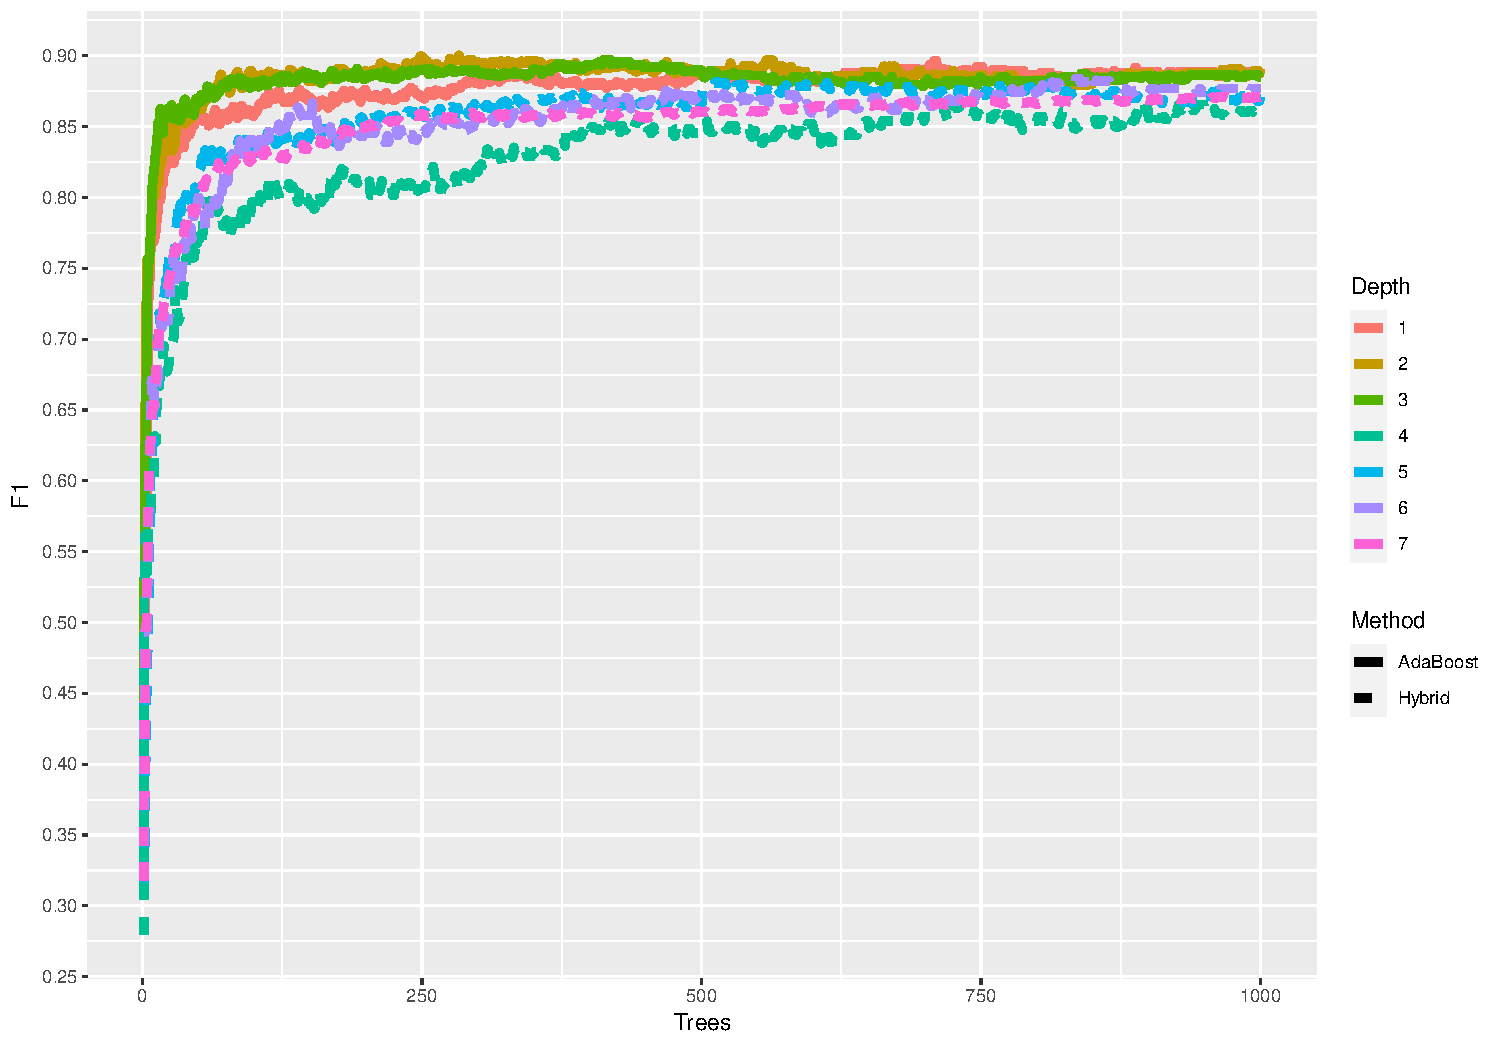
\includegraphics[width=0.8\textwidth]{media/depth.pdf}}
    \caption{
        \raggedright
        A comparison of F1 scores across different max tree depths, methods and forest size.\label{depth_cmp}
    }
\end{figure}
\section{The impact of feature sources\label{feature-results}}
\chapter{Conclusion}

\bibliographystyle{apacite}
\linespread{1}
\raggedright
\bibliography{references.bib}

\end{document}

\documentclass[12pt]{article}
\usepackage{hyperref} % For links
\usepackage{tikz} % For drawing stuff.
\usepackage{qtree} % For drawing trees (needs tikz).
\usepackage{setspace} % For going between double lines and single.
\usepackage[a4paper, total={5.7in, 8in}]{geometry} % Setting margin.
\usepackage{subfiles} % Splitting work across files.
\usepackage{apacite} % Referencing, duh.

\newcommand{\nr}{{\tt newsreduce.org}}
\newcommand{\pr}{PR}

\newcounter{nodeCdepth}%
\newenvironment{nodeC}%
  {\ifnum\value{nodeCdepth}=0%
     \gdef\listfordirtree{}%
     \let\item\nodeCitem%
    \fi%
    \stepcounter{nodeCdepth}}%
  {\addtocounter{nodeCdepth}{-1}%
   \ifnum\value{nodeCdepth}=0%
     \expandafter\dirtree\expandafter{\listfordirtree}%
   \fi}%
\newcommand{\nodeCitem}[1]{%
  \xdef\listfordirtree{%
    \unexpanded\expandafter{\listfordirtree}%
    .\thenodeCdepth\space\unexpanded{#1}. }%
}%

\algnewcommand\algorithmicforeach{\textbf{for each}}
\algdef{S}[FOR]{ForEach}[1]{\algorithmicforeach\ #1\ \algorithmicdo}

\doublespacing

\title{\nr{}
\\
A personalised and privacy-respecting newsreader}
\author{Seán Healy }
\date{August 2020}

\begin{document}

\maketitle
\begin{abstract}
\noindent A web-based newsreader is designed and implemented using a cocktail
of software engineering, natural language processing and machine
learning techniques.  The newsreader aims to tackle some issues
in the current newsreader space: user privacy concerns, information
overload, advertising influence and low coverage.
\end{abstract}
\section*{Acknowledgements}
I must thank Dr. Kevin Koidl for his valuable advice and
help throughout my dissertation.  I must also thank Visma (my
employer) for granting me three months leave in order to complete
this large project and dissertation.
\tableofcontents

\documentclass[12pt]{article}
\usepackage{hyperref} % For links
\usepackage{tikz} % For drawing stuff.
\usepackage{qtree} % For drawing trees (needs tikz).
\usepackage{setspace} % For going between double lines and single.
\usepackage[a4paper, total={5.7in, 8in}]{geometry} % Setting margin.
\usepackage{subfiles} % Splitting work across files.
\usepackage{apacite} % Referencing, duh.

\include{shortcuts}

\doublespacing

\title{\nr{}
\\
A personalised and privacy-respecting newsreader}
\author{Seán Healy }
\date{August 2020}

\begin{document}

\maketitle
\include{abstract}
\include{acknowledge}
\tableofcontents

\include{1-intro/main}
\include{2-background/main}
\include{3-method/main}
\include{4-results}
\include{5-conclusion}

\bibliographystyle{apacite}
\linespread{1}
\raggedright
\bibliography{references.bib}

\end{document}

\documentclass[12pt]{article}
\usepackage{hyperref} % For links
\usepackage{tikz} % For drawing stuff.
\usepackage{qtree} % For drawing trees (needs tikz).
\usepackage{setspace} % For going between double lines and single.
\usepackage[a4paper, total={5.7in, 8in}]{geometry} % Setting margin.
\usepackage{subfiles} % Splitting work across files.
\usepackage{apacite} % Referencing, duh.

\include{shortcuts}

\doublespacing

\title{\nr{}
\\
A personalised and privacy-respecting newsreader}
\author{Seán Healy }
\date{August 2020}

\begin{document}

\maketitle
\include{abstract}
\include{acknowledge}
\tableofcontents

\include{1-intro/main}
\include{2-background/main}
\include{3-method/main}
\include{4-results}
\include{5-conclusion}

\bibliographystyle{apacite}
\linespread{1}
\raggedright
\bibliography{references.bib}

\end{document}

\documentclass[12pt]{article}
\usepackage{hyperref} % For links
\usepackage{tikz} % For drawing stuff.
\usepackage{qtree} % For drawing trees (needs tikz).
\usepackage{setspace} % For going between double lines and single.
\usepackage[a4paper, total={5.7in, 8in}]{geometry} % Setting margin.
\usepackage{subfiles} % Splitting work across files.
\usepackage{apacite} % Referencing, duh.

\include{shortcuts}

\doublespacing

\title{\nr{}
\\
A personalised and privacy-respecting newsreader}
\author{Seán Healy }
\date{August 2020}

\begin{document}

\maketitle
\include{abstract}
\include{acknowledge}
\tableofcontents

\include{1-intro/main}
\include{2-background/main}
\include{3-method/main}
\include{4-results}
\include{5-conclusion}

\bibliographystyle{apacite}
\linespread{1}
\raggedright
\bibliography{references.bib}

\end{document}

\chapter{Results and discussion\label{results}}
\section{Comparison of resource models\label{model-results}}
\section{Comparison of classifiers\label{classifier-results}}
\begin{figure}[H]
    \centering
    \fbox{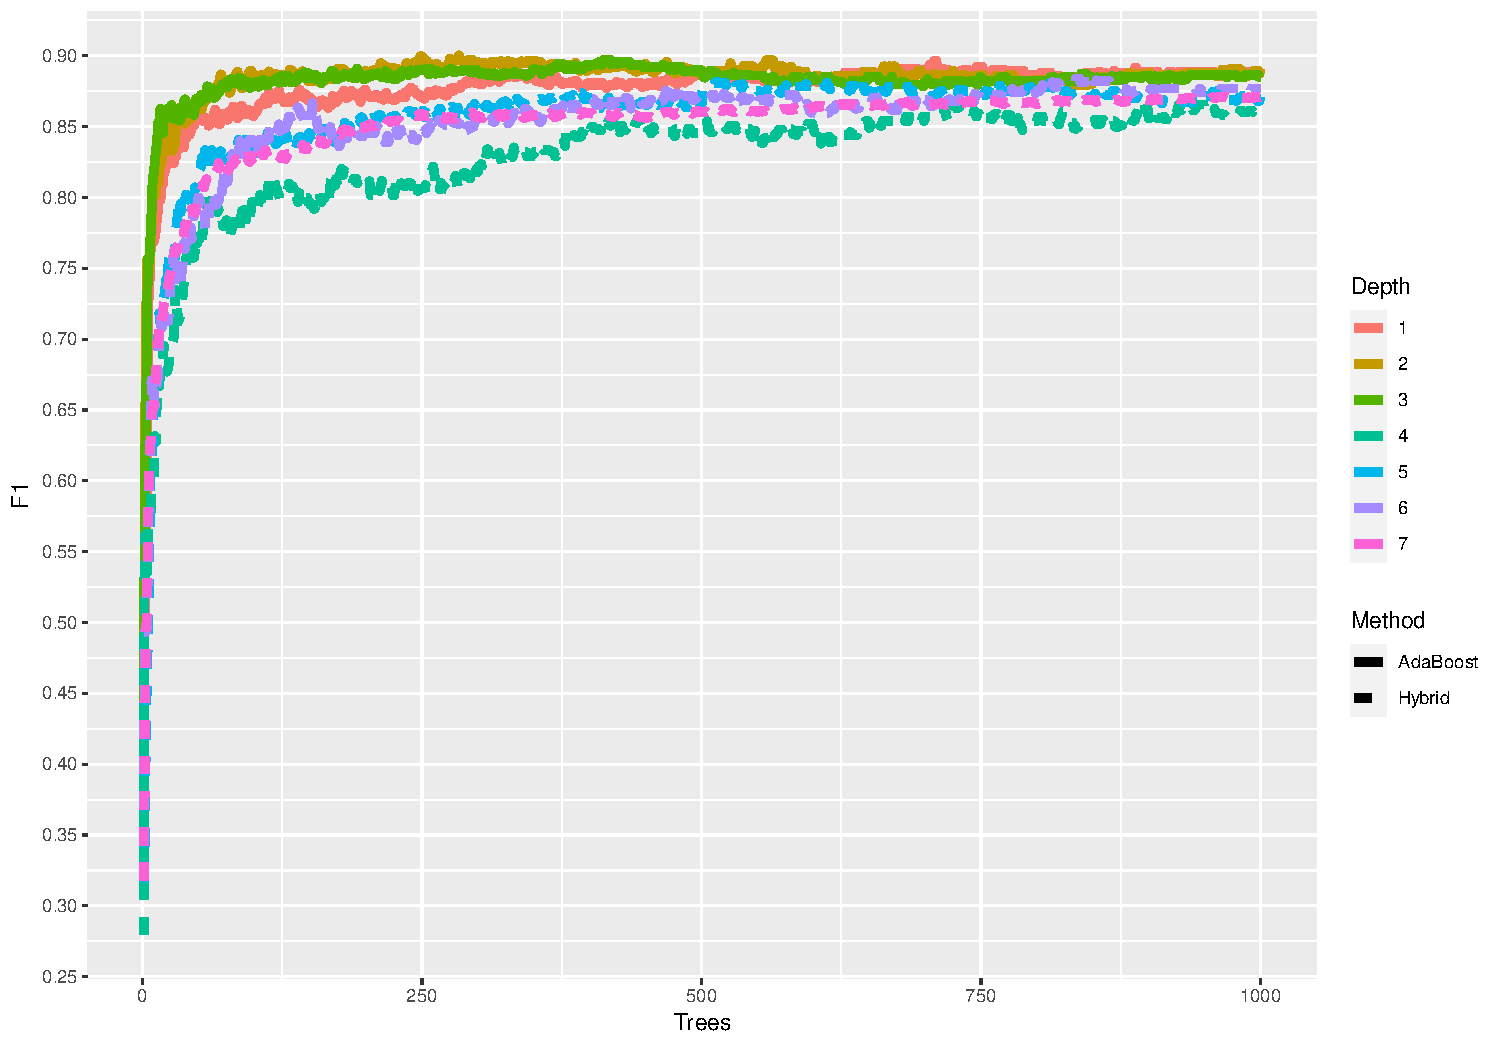
\includegraphics[width=0.8\textwidth]{media/depth.pdf}}
    \caption{
        \raggedright
        A comparison of F1 scores across different max tree depths, methods and forest size.\label{depth_cmp}
    }
\end{figure}
\section{The impact of feature sources\label{feature-results}}
\chapter{Conclusion}

\bibliographystyle{apacite}
\linespread{1}
\raggedright
\bibliography{references.bib}

\end{document}

\documentclass[12pt]{article}
\usepackage{hyperref} % For links
\usepackage{tikz} % For drawing stuff.
\usepackage{qtree} % For drawing trees (needs tikz).
\usepackage{setspace} % For going between double lines and single.
\usepackage[a4paper, total={5.7in, 8in}]{geometry} % Setting margin.
\usepackage{subfiles} % Splitting work across files.
\usepackage{apacite} % Referencing, duh.

\newcommand{\nr}{{\tt newsreduce.org}}
\newcommand{\pr}{PR}

\newcounter{nodeCdepth}%
\newenvironment{nodeC}%
  {\ifnum\value{nodeCdepth}=0%
     \gdef\listfordirtree{}%
     \let\item\nodeCitem%
    \fi%
    \stepcounter{nodeCdepth}}%
  {\addtocounter{nodeCdepth}{-1}%
   \ifnum\value{nodeCdepth}=0%
     \expandafter\dirtree\expandafter{\listfordirtree}%
   \fi}%
\newcommand{\nodeCitem}[1]{%
  \xdef\listfordirtree{%
    \unexpanded\expandafter{\listfordirtree}%
    .\thenodeCdepth\space\unexpanded{#1}. }%
}%

\algnewcommand\algorithmicforeach{\textbf{for each}}
\algdef{S}[FOR]{ForEach}[1]{\algorithmicforeach\ #1\ \algorithmicdo}

\doublespacing

\title{\nr{}
\\
A personalised and privacy-respecting newsreader}
\author{Seán Healy }
\date{August 2020}

\begin{document}

\maketitle
\begin{abstract}
\noindent A web-based newsreader is designed and implemented using a cocktail
of software engineering, natural language processing and machine
learning techniques.  The newsreader aims to tackle some issues
in the current newsreader space: user privacy concerns, information
overload, advertising influence and low coverage.
\end{abstract}
\section*{Acknowledgements}
I must thank Dr. Kevin Koidl for his valuable advice and
help throughout my dissertation.  I must also thank Visma (my
employer) for granting me three months leave in order to complete
this large project and dissertation.
\tableofcontents

\documentclass[12pt]{article}
\usepackage{hyperref} % For links
\usepackage{tikz} % For drawing stuff.
\usepackage{qtree} % For drawing trees (needs tikz).
\usepackage{setspace} % For going between double lines and single.
\usepackage[a4paper, total={5.7in, 8in}]{geometry} % Setting margin.
\usepackage{subfiles} % Splitting work across files.
\usepackage{apacite} % Referencing, duh.

\include{shortcuts}

\doublespacing

\title{\nr{}
\\
A personalised and privacy-respecting newsreader}
\author{Seán Healy }
\date{August 2020}

\begin{document}

\maketitle
\include{abstract}
\include{acknowledge}
\tableofcontents

\include{1-intro/main}
\include{2-background/main}
\include{3-method/main}
\include{4-results}
\include{5-conclusion}

\bibliographystyle{apacite}
\linespread{1}
\raggedright
\bibliography{references.bib}

\end{document}

\documentclass[12pt]{article}
\usepackage{hyperref} % For links
\usepackage{tikz} % For drawing stuff.
\usepackage{qtree} % For drawing trees (needs tikz).
\usepackage{setspace} % For going between double lines and single.
\usepackage[a4paper, total={5.7in, 8in}]{geometry} % Setting margin.
\usepackage{subfiles} % Splitting work across files.
\usepackage{apacite} % Referencing, duh.

\include{shortcuts}

\doublespacing

\title{\nr{}
\\
A personalised and privacy-respecting newsreader}
\author{Seán Healy }
\date{August 2020}

\begin{document}

\maketitle
\include{abstract}
\include{acknowledge}
\tableofcontents

\include{1-intro/main}
\include{2-background/main}
\include{3-method/main}
\include{4-results}
\include{5-conclusion}

\bibliographystyle{apacite}
\linespread{1}
\raggedright
\bibliography{references.bib}

\end{document}

\documentclass[12pt]{article}
\usepackage{hyperref} % For links
\usepackage{tikz} % For drawing stuff.
\usepackage{qtree} % For drawing trees (needs tikz).
\usepackage{setspace} % For going between double lines and single.
\usepackage[a4paper, total={5.7in, 8in}]{geometry} % Setting margin.
\usepackage{subfiles} % Splitting work across files.
\usepackage{apacite} % Referencing, duh.

\include{shortcuts}

\doublespacing

\title{\nr{}
\\
A personalised and privacy-respecting newsreader}
\author{Seán Healy }
\date{August 2020}

\begin{document}

\maketitle
\include{abstract}
\include{acknowledge}
\tableofcontents

\include{1-intro/main}
\include{2-background/main}
\include{3-method/main}
\include{4-results}
\include{5-conclusion}

\bibliographystyle{apacite}
\linespread{1}
\raggedright
\bibliography{references.bib}

\end{document}

\chapter{Results and discussion\label{results}}
\section{Comparison of resource models\label{model-results}}
\section{Comparison of classifiers\label{classifier-results}}
\begin{figure}[H]
    \centering
    \fbox{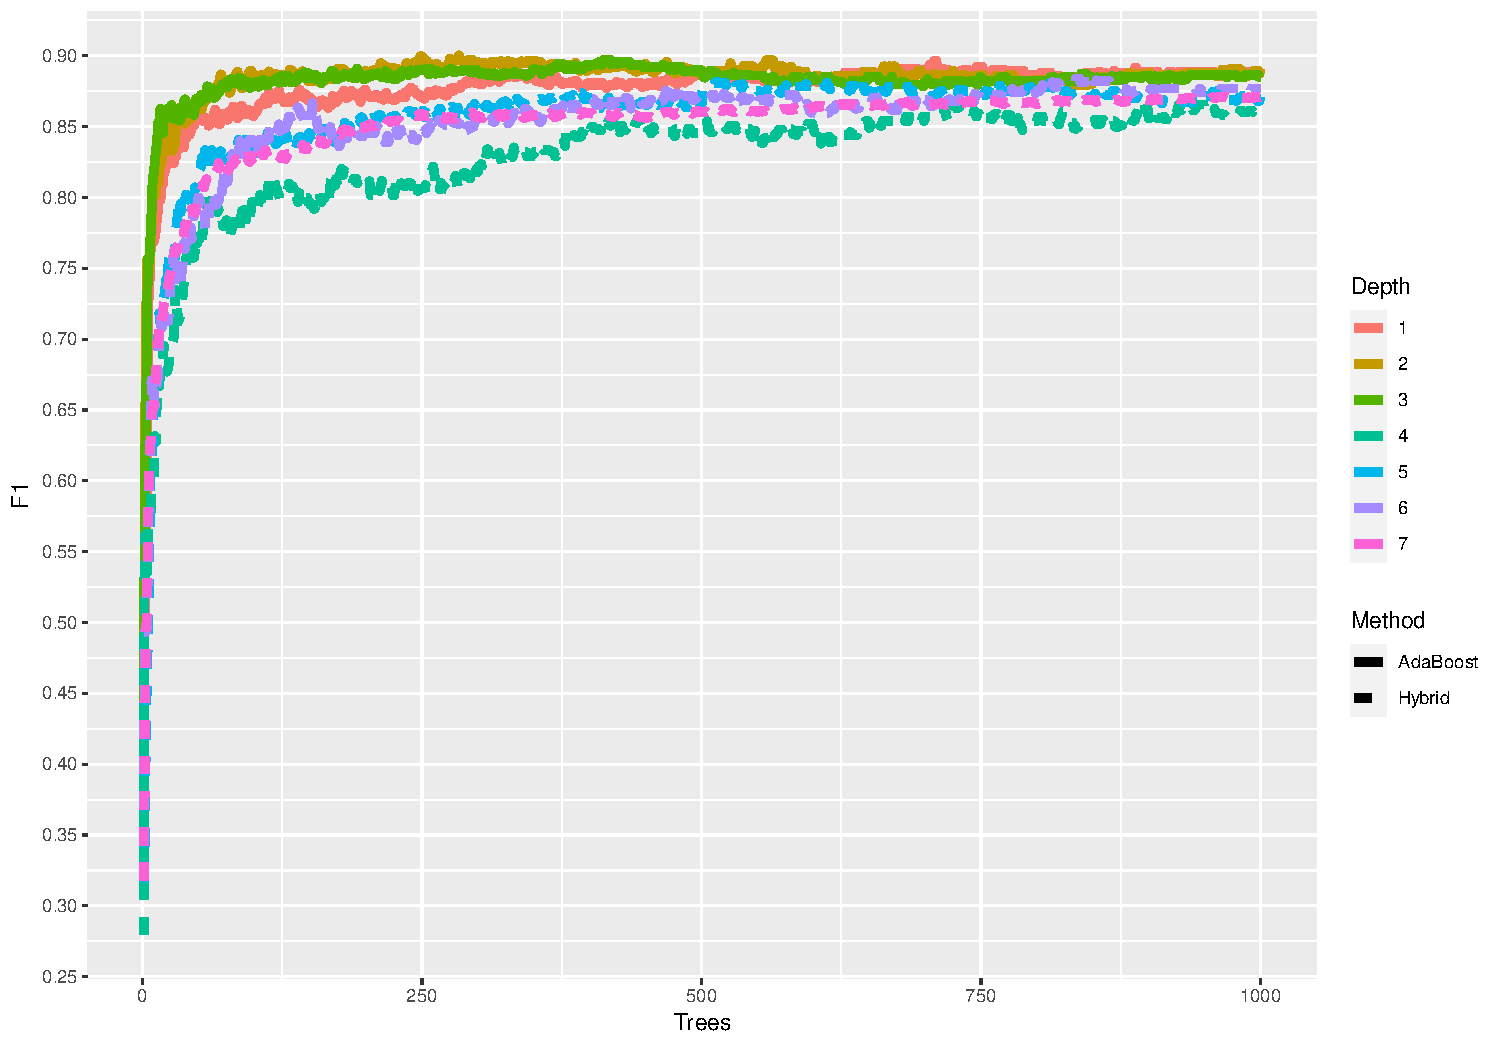
\includegraphics[width=0.8\textwidth]{media/depth.pdf}}
    \caption{
        \raggedright
        A comparison of F1 scores across different max tree depths, methods and forest size.\label{depth_cmp}
    }
\end{figure}
\section{The impact of feature sources\label{feature-results}}
\chapter{Conclusion}

\bibliographystyle{apacite}
\linespread{1}
\raggedright
\bibliography{references.bib}

\end{document}

\chapter{Results and discussion\label{results}}
\section{Comparison of resource models\label{model-results}}
\section{Comparison of classifiers\label{classifier-results}}
\begin{figure}[H]
    \centering
    \fbox{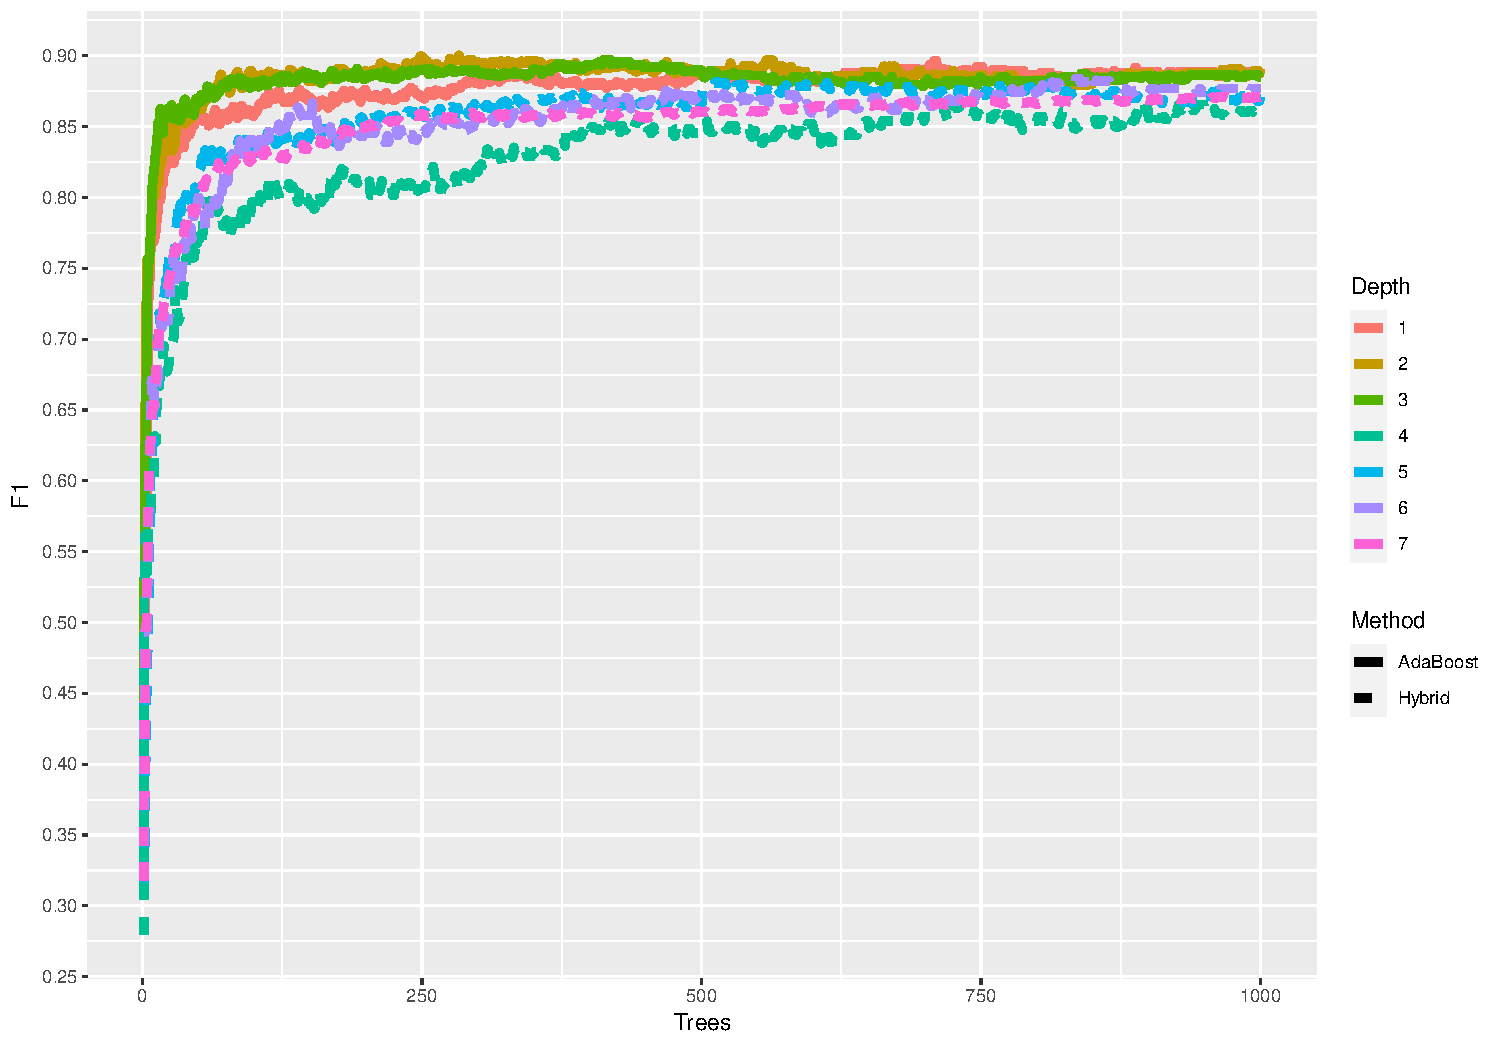
\includegraphics[width=0.8\textwidth]{media/depth.pdf}}
    \caption{
        \raggedright
        A comparison of F1 scores across different max tree depths, methods and forest size.\label{depth_cmp}
    }
\end{figure}
\section{The impact of feature sources\label{feature-results}}
\chapter{Conclusion}

\bibliographystyle{apacite}
\linespread{1}
\raggedright
\bibliography{references.bib}

\end{document}

\chapter{Results and discussion\label{results}}
\section{Comparison of resource models\label{model-results}}
\section{Comparison of classifiers\label{classifier-results}}
\begin{figure}[H]
    \centering
    \fbox{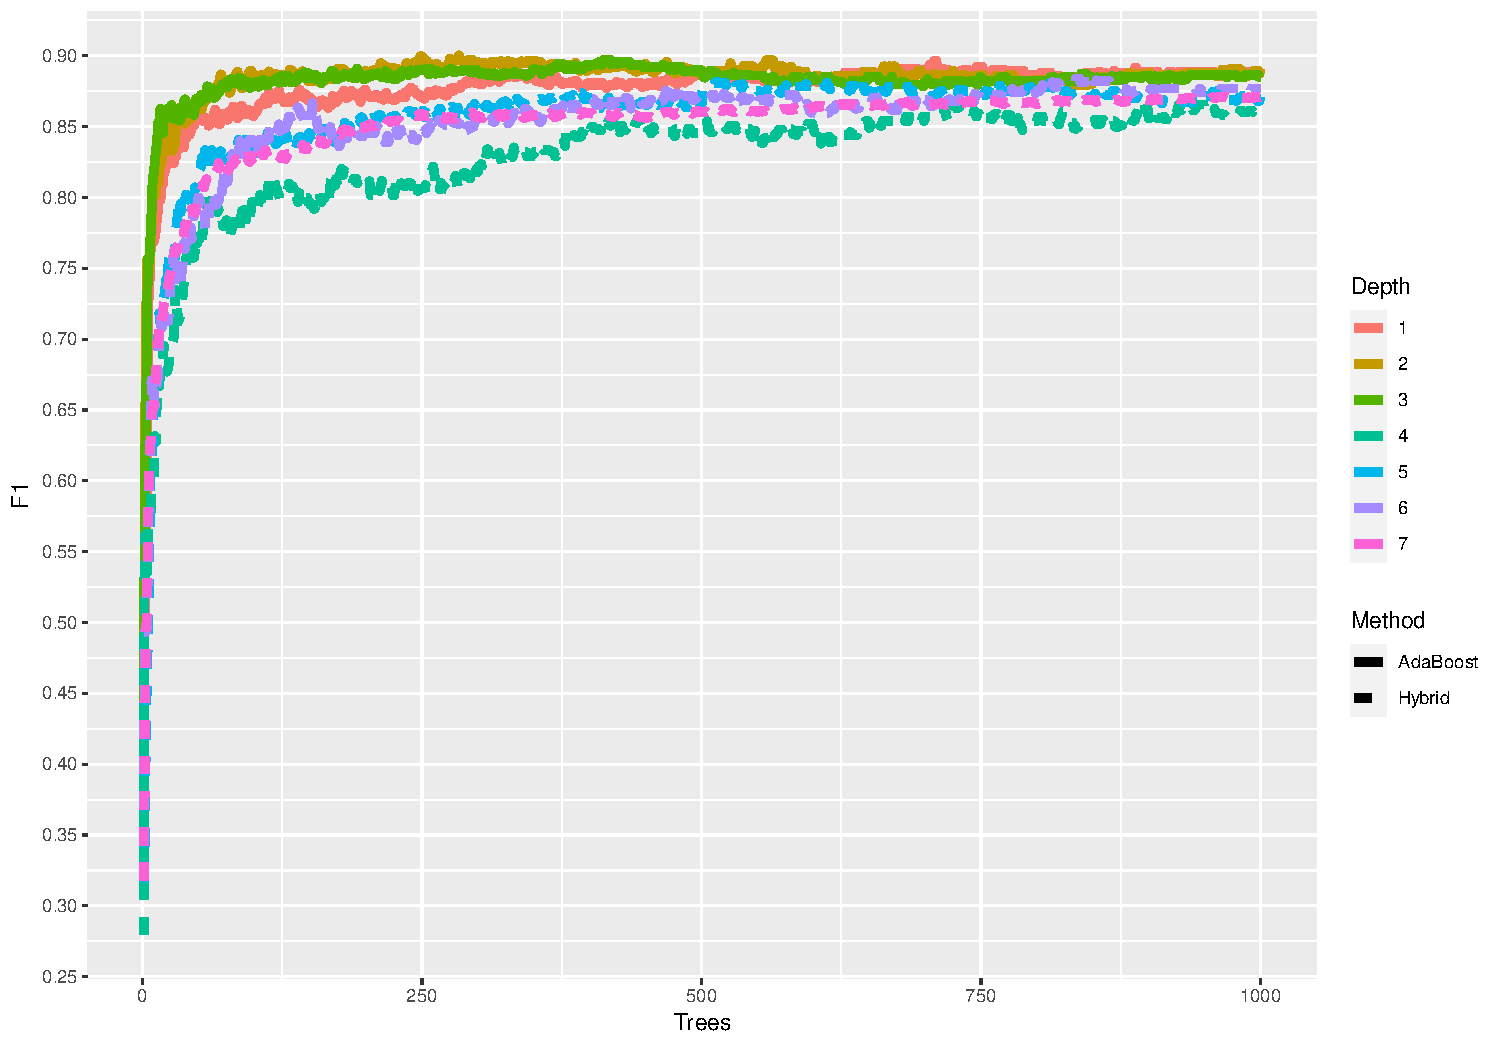
\includegraphics[width=0.8\textwidth]{media/depth.pdf}}
    \caption{
        \raggedright
        A comparison of F1 scores across different max tree depths, methods and forest size.\label{depth_cmp}
    }
\end{figure}
\section{The impact of feature sources\label{feature-results}}
\chapter{Conclusion}

\bibliographystyle{apacite}
\linespread{1}
\raggedright
\bibliography{references.bib}

\end{document}
